\documentclass[american,]{article}
\usepackage{lmodern}
\usepackage{amssymb,amsmath}
\usepackage{ifxetex,ifluatex}
\usepackage{fixltx2e} % provides \textsubscript
\ifnum 0\ifxetex 1\fi\ifluatex 1\fi=0 % if pdftex
  \usepackage[T1]{fontenc}
  \usepackage[utf8]{inputenc}
\else % if luatex or xelatex
  \ifxetex
    \usepackage{mathspec}
  \else
    \usepackage{fontspec}
  \fi
  \defaultfontfeatures{Ligatures=TeX,Scale=MatchLowercase}
\fi
% use upquote if available, for straight quotes in verbatim environments
\IfFileExists{upquote.sty}{\usepackage{upquote}}{}
% use microtype if available
\IfFileExists{microtype.sty}{%
\usepackage{microtype}
\UseMicrotypeSet[protrusion]{basicmath} % disable protrusion for tt fonts
}{}
\usepackage[margin=2cm]{geometry}
\usepackage{hyperref}
\hypersetup{unicode=true,
            pdfborder={0 0 0},
            breaklinks=true}
\urlstyle{same}  % don't use monospace font for urls
\ifnum 0\ifxetex 1\fi\ifluatex 1\fi=0 % if pdftex
  \usepackage[shorthands=off,main=american]{babel}
\else
  \usepackage{polyglossia}
  \setmainlanguage[variant=american]{english}
\fi
\usepackage{color}
\usepackage{fancyvrb}
\newcommand{\VerbBar}{|}
\newcommand{\VERB}{\Verb[commandchars=\\\{\}]}
\DefineVerbatimEnvironment{Highlighting}{Verbatim}{commandchars=\\\{\}}
% Add ',fontsize=\small' for more characters per line
\usepackage{framed}
\definecolor{shadecolor}{RGB}{248,248,248}
\newenvironment{Shaded}{\begin{snugshade}}{\end{snugshade}}
\newcommand{\AlertTok}[1]{\textcolor[rgb]{0.94,0.16,0.16}{#1}}
\newcommand{\AnnotationTok}[1]{\textcolor[rgb]{0.56,0.35,0.01}{\textbf{\textit{#1}}}}
\newcommand{\AttributeTok}[1]{\textcolor[rgb]{0.77,0.63,0.00}{#1}}
\newcommand{\BaseNTok}[1]{\textcolor[rgb]{0.00,0.00,0.81}{#1}}
\newcommand{\BuiltInTok}[1]{#1}
\newcommand{\CharTok}[1]{\textcolor[rgb]{0.31,0.60,0.02}{#1}}
\newcommand{\CommentTok}[1]{\textcolor[rgb]{0.56,0.35,0.01}{\textit{#1}}}
\newcommand{\CommentVarTok}[1]{\textcolor[rgb]{0.56,0.35,0.01}{\textbf{\textit{#1}}}}
\newcommand{\ConstantTok}[1]{\textcolor[rgb]{0.00,0.00,0.00}{#1}}
\newcommand{\ControlFlowTok}[1]{\textcolor[rgb]{0.13,0.29,0.53}{\textbf{#1}}}
\newcommand{\DataTypeTok}[1]{\textcolor[rgb]{0.13,0.29,0.53}{#1}}
\newcommand{\DecValTok}[1]{\textcolor[rgb]{0.00,0.00,0.81}{#1}}
\newcommand{\DocumentationTok}[1]{\textcolor[rgb]{0.56,0.35,0.01}{\textbf{\textit{#1}}}}
\newcommand{\ErrorTok}[1]{\textcolor[rgb]{0.64,0.00,0.00}{\textbf{#1}}}
\newcommand{\ExtensionTok}[1]{#1}
\newcommand{\FloatTok}[1]{\textcolor[rgb]{0.00,0.00,0.81}{#1}}
\newcommand{\FunctionTok}[1]{\textcolor[rgb]{0.00,0.00,0.00}{#1}}
\newcommand{\ImportTok}[1]{#1}
\newcommand{\InformationTok}[1]{\textcolor[rgb]{0.56,0.35,0.01}{\textbf{\textit{#1}}}}
\newcommand{\KeywordTok}[1]{\textcolor[rgb]{0.13,0.29,0.53}{\textbf{#1}}}
\newcommand{\NormalTok}[1]{#1}
\newcommand{\OperatorTok}[1]{\textcolor[rgb]{0.81,0.36,0.00}{\textbf{#1}}}
\newcommand{\OtherTok}[1]{\textcolor[rgb]{0.56,0.35,0.01}{#1}}
\newcommand{\PreprocessorTok}[1]{\textcolor[rgb]{0.56,0.35,0.01}{\textit{#1}}}
\newcommand{\RegionMarkerTok}[1]{#1}
\newcommand{\SpecialCharTok}[1]{\textcolor[rgb]{0.00,0.00,0.00}{#1}}
\newcommand{\SpecialStringTok}[1]{\textcolor[rgb]{0.31,0.60,0.02}{#1}}
\newcommand{\StringTok}[1]{\textcolor[rgb]{0.31,0.60,0.02}{#1}}
\newcommand{\VariableTok}[1]{\textcolor[rgb]{0.00,0.00,0.00}{#1}}
\newcommand{\VerbatimStringTok}[1]{\textcolor[rgb]{0.31,0.60,0.02}{#1}}
\newcommand{\WarningTok}[1]{\textcolor[rgb]{0.56,0.35,0.01}{\textbf{\textit{#1}}}}
\usepackage{longtable,booktabs}
\usepackage{graphicx}
% grffile has become a legacy package: https://ctan.org/pkg/grffile
\IfFileExists{grffile.sty}{%
\usepackage{grffile}
}{}
\makeatletter
\def\maxwidth{\ifdim\Gin@nat@width>\linewidth\linewidth\else\Gin@nat@width\fi}
\def\maxheight{\ifdim\Gin@nat@height>\textheight\textheight\else\Gin@nat@height\fi}
\makeatother
% Scale images if necessary, so that they will not overflow the page
% margins by default, and it is still possible to overwrite the defaults
% using explicit options in \includegraphics[width, height, ...]{}
\setkeys{Gin}{width=\maxwidth,height=\maxheight,keepaspectratio}
\IfFileExists{parskip.sty}{%
\usepackage{parskip}
}{% else
\setlength{\parindent}{0pt}
\setlength{\parskip}{6pt plus 2pt minus 1pt}
}
\setlength{\emergencystretch}{3em}  % prevent overfull lines
\providecommand{\tightlist}{%
  \setlength{\itemsep}{0pt}\setlength{\parskip}{0pt}}
\setcounter{secnumdepth}{5}
% Redefines (sub)paragraphs to behave more like sections
\ifx\paragraph\undefined\else
\let\oldparagraph\paragraph
\renewcommand{\paragraph}[1]{\oldparagraph{#1}\mbox{}}
\fi
\ifx\subparagraph\undefined\else
\let\oldsubparagraph\subparagraph
\renewcommand{\subparagraph}[1]{\oldsubparagraph{#1}\mbox{}}
\fi

%%% Use protect on footnotes to avoid problems with footnotes in titles
\let\rmarkdownfootnote\footnote%
\def\footnote{\protect\rmarkdownfootnote}

%%% Change title format to be more compact
\usepackage{titling}

% Create subtitle command for use in maketitle
\providecommand{\subtitle}[1]{
  \posttitle{
    \begin{center}\large#1\end{center}
    }
}

\setlength{\droptitle}{-2em}

  \title{}
    \pretitle{\vspace{\droptitle}}
  \posttitle{}
    \author{}
    \preauthor{}\postauthor{}
    \date{}
    \predate{}\postdate{}
  
\usepackage{booktabs}
\usepackage{longtable}
\usepackage{array}
\usepackage{multirow}
\usepackage{wrapfig}
\usepackage{float}
\usepackage{colortbl}
\usepackage{pdflscape}
\usepackage{tabu}
\usepackage{threeparttable}
\usepackage{threeparttablex}
\usepackage[normalem]{ulem}
\usepackage{makecell}
\usepackage{xcolor}

\usepackage{float}

\begin{document}

{
\setcounter{tocdepth}{2}
\tableofcontents
}
\newpage

\hypertarget{abstract}{%
\section{\texorpdfstring{\textbf{Abstract:}}{Abstract:}}\label{abstract}}

\emph{This project investigates the correlation between multiple potential explanatory variables and Kobe Bryant's ability to make a shot while playing for the NBA team Los Angeles Lakers using data gathered from \texttt{1996}-\texttt{2015}.}

\hypertarget{introduction}{%
\section{\texorpdfstring{\textbf{Introduction}}{Introduction}}\label{introduction}}

Kobe Bryant, a professional basketball player, spent his entire 20-year career with one team, the LA Lakers as a guard. Bryant started with the Lakers just after high school and went on to win five NBA Championships and 18 All-Star titles. Kobe Bryant's career average points scored per game is 25-points during the regular season and 26-points during playoffs. In addition to these statistics, using the \texttt{KobeData} provided, we were able to determine the odds of Kobe making a shot decreases with respect to his distance from the hoop and the probability of him making a shot decreases after taking into consideration his distance from the hoop and analyze the relationship distance and making a shot during the playoffs. During model selection we considered Area Under the Curve (AUC), Mis-Classification Rate, Sensitivity, Specificity and objective / loss function when making model comparisons.

\hypertarget{exploratory-data-analysis}{%
\section{\texorpdfstring{\textbf{Exploratory Data Analysis}}{Exploratory Data Analysis}}\label{exploratory-data-analysis}}

\hypertarget{outlier-check-transformations}{%
\subsection{\texorpdfstring{\textbf{Outlier Check \& Transformations}}{Outlier Check \& Transformations}}\label{outlier-check-transformations}}

First, we performed a brief outlier check, which included a graphical analysis of all shots taken, by loc\_x and loc\_y. This graphical analysis indicated a 2PT (2-point) Field Goal was recorded from the 3PT (3-point) range. Upon inspection of other attributes - such as action type and shot\_zone\_range - we verified this shot to be a member member of the 3-point level of shot\_type. Under the assumption shots from beyond the 300 inch mark are more likely to have been incorrectly recorded as 2 points rather than an incorrectly recorded location y, we modified our programming to transform all shots where \(loc_y > 300\) to be recoded as \texttt{3PT\ Field\ Gloal}.

Additionally, \texttt{action\_type} was recoded where shots types were categorized into \texttt{short} and \texttt{not\_short}. However, modeling performance decreased because the parameter became less descriptive. Further transformations included using indicator variables for \texttt{shot\_made\_flag}, depending on the phase of analysis and modeling.

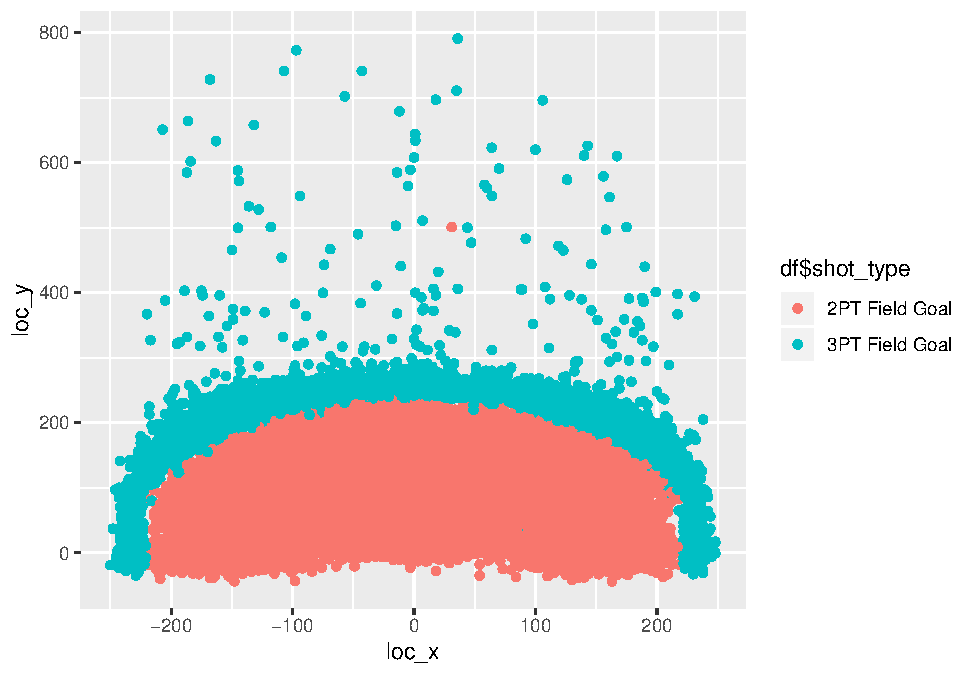
\includegraphics{Final_Project_Applied_files/figure-latex/outlier check-1.pdf}

\hypertarget{variable-elimination}{%
\subsection{\texorpdfstring{\textbf{Variable Elimination}}{Variable Elimination}}\label{variable-elimination}}

Next, we removed one-level factors. These will never change so are not useful to the model; including can cause issues with model sensitivity since linear trajectories will be down-weighted. Therefore, their significance will be lessened by the constant state of the additional parameters. While this is may not be significant, it is not condusive to model quality.

\hypertarget{addressing-multicollinearity-correlation-heat-map-for-visual-data-exploration}{%
\subsection{\texorpdfstring{\textbf{Addressing Multicollinearity: Correlation Heat Map for Visual Data Exploration}}{Addressing Multicollinearity: Correlation Heat Map for Visual Data Exploration}}\label{addressing-multicollinearity-correlation-heat-map-for-visual-data-exploration}}

To address multicollinearity among quantitative predictor variables, a correlation heat map (below) was created for visual inspection of correlation. Red corresponds to negative correlation (where an increase in a predictor causes a decrease in the value of its collinear counterpart) whereas blue corresponds to positive correlation.
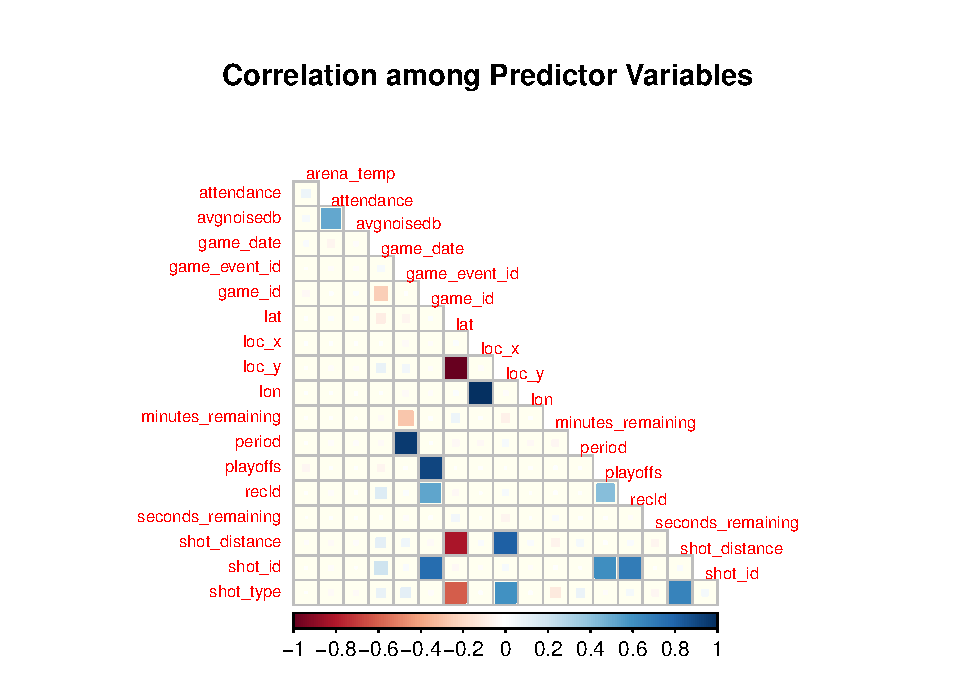
\includegraphics{Final_Project_Applied_files/figure-latex/Multicollinearity-1.pdf}

\hypertarget{post-correlation-heat-map-variable-elimination}{%
\subsection{\texorpdfstring{\textbf{Post-Correlation Heat Map Variable Elimination}}{Post-Correlation Heat Map Variable Elimination}}\label{post-correlation-heat-map-variable-elimination}}

Following our correlation heat map, we decided to eliminate some collinear terms. However, some of the collinearity is useful to capture the instances where the terms are unique. For example, \texttt{combined\_shot\_type} (factor variable) is collinear with \texttt{shot\_distance} (quantitative variable), but it also accounts for the method Kobe may use to take a shot. For example, distance may be relatively the same between 10 and 11 feet, but the factor levels used to derrive their \texttt{short} or \texttt{far} indications may differ. This difference could be whether Kobe makes a potentially more accurate heel-planted shot or if he is forced to lean forward and take a riskier shot at basket; the difference in distance may only be one foot, but the difference in technique could measure significant relative to the odds of success. Because this is a healthy level of confusion for the model, some multicollinearity was accepted.

\hypertarget{addressing-multicollinearity-correlation-matrix-for-numerical-analysis}{%
\subsection{\texorpdfstring{\textbf{Addressing Multicollinearity: Correlation Matrix for Numerical Analysis}}{Addressing Multicollinearity: Correlation Matrix for Numerical Analysis}}\label{addressing-multicollinearity-correlation-matrix-for-numerical-analysis}}

After deselecting the most obvious collinear terms through visually inspection of the correlation plot, a correlation matrix for analyzing the remaining results. Collinear quantitative data was preliminarily removed following correlation plot analysis to desaturate the model to an extent that allows more distinction among significance measures for terms in the correlation matrix. Following the removal of predictor variables after visually inspecting the correlation heat map, we analyzed a correlation matrix. However, the matrix itself did not identify any remaining collinearity at a threshold of correlation necessitating removal of like-terms. Consequently, no further predictor variables are removed. Please refer to the table below for a list of the remaining top 10 collinear terms following first-pass variable removal. While this risks over-fitting, we believed the variables were different enough to capture useful information for the model.

The Variance Inflation Factor (VIF) scores across all remaining variables is another test applied in consideration for multicollinearity among explanatory variables. A threshold of roughly 1 or higher is considered a strong level of collinearity. Both VIF and correlation matrix statistics were considered during model development.

\hypertarget{top-10-multicollinear-terms-correlation-matrix}{%
\subsubsection{\texorpdfstring{\textbf{Top 10 Multicollinear Terms, Correlation Matrix:}}{Top 10 Multicollinear Terms, Correlation Matrix:}}\label{top-10-multicollinear-terms-correlation-matrix}}

\begin{table}[H]
\centering
\begin{tabular}{llrl}
\toprule
Correlation Predictor Variable & Correlation Response Variable & Correlation & p-Value\\
\midrule
\rowcolor{gray!6}  loc\_y & shot\_distance & 0.81812 & p < 0.0001\\
recId & shot\_id & 0.69172 & p < 0.0001\\
\rowcolor{gray!6}  shot\_distance & shot\_type & 0.66861 & p < 0.0001\\
playoffs & shot\_id & 0.61299 & p < 0.0001\\
\rowcolor{gray!6}  loc\_y & shot\_type & 0.60662 & p < 0.0001\\
\addlinespace
attendance & avgnoisedb & 0.51092 & p < 0.0001\\
\rowcolor{gray!6}  recId & playoffs & 0.42527 & p < 0.0001\\
game\_date & shot\_id & 0.20932 & p < 0.0001\\
\rowcolor{gray!6}  recId & game\_date & 0.14773 & p < 0.0001\\
game\_event\_id & shot\_type & 0.11238 & p < 0.0001\\
\bottomrule
\end{tabular}
\end{table}

\hypertarget{top-10-multicollinear-terms-variance-inflation-factor}{%
\subsubsection{\texorpdfstring{\textbf{Top 10 Multicollinear Terms, Variance Inflation Factor:}}{Top 10 Multicollinear Terms, Variance Inflation Factor:}}\label{top-10-multicollinear-terms-variance-inflation-factor}}

\begin{table}[H]
\centering
\begin{tabular}{lr}
\toprule
Variable & Variance Inflation Factor\\
\midrule
\rowcolor{gray!6}  shot\_id & 41103299.94\\
recId & 41101644.14\\
\rowcolor{gray!6}  shot\_distance & 3.75\\
loc\_y & 3.31\\
\rowcolor{gray!6}  shot\_type & 1.88\\
\addlinespace
playoffs & 1.78\\
\rowcolor{gray!6}  game\_event\_id & 1.60\\
\bottomrule
\end{tabular}
\end{table}

\hypertarget{quadratic-discriminant-analysis}{%
\section{\texorpdfstring{\textbf{Quadratic Discriminant Analysis}}{Quadratic Discriminant Analysis}}\label{quadratic-discriminant-analysis}}

As requested within the requirements of this study, a Linear Discriminant Analysis must be assessed and provided. Discriminant analysis is an operation that compares a categorical response variable against measures of quantitative predictor variables. As a result, analysis for this section is performed on the numerical predictors, which include \texttt{recId}, \texttt{game\_event\_id}, \texttt{game\_id}, \texttt{loc\_x}, \texttt{loc\_y}, \texttt{minutes\_remaining}, \texttt{seconds\_remaining}, \texttt{shot\_distance}, \texttt{shot\_made\_flag}, \texttt{shot\_type}, \texttt{game\_date}, \texttt{shot\_id}, \texttt{attendance}, \texttt{arena\_temp}, \texttt{avgnoisedb}, controlling collinearity by eliminating a member of each collinear pair prior to model development.

\texttt{Linear\ Discriminant\ Analysis} requires a linear boundary between the predictor variables, respective of the response. If the boundary between predictors and response is not linear, \texttt{Quadratic\ Discriminant\ Analysis} (QDA) must be used. \texttt{Wilks\textquotesingle{}\ Lambda} distribution is used to assess the nature of boundary linearity, which is a required understanding to develop a well-fit discriminant classification model. However, because of the large dimensions of the data set analyzed in this study, an approximation of Wilks' Lambda must be used, rather than Wilks' Lambda itself. \texttt{Bartlett\textquotesingle{}s\ Test} is an approximation of Wilks' Lambda that can be used for models with large dimensions by applying a measure against the \texttt{Chi-Square\ distribution}. This method is applied herein to assess linearity.

Also to note of importance, \texttt{a\ priori} knowledge was set to the default proportions when performing Quadratic Discriminant Analysis.

\hypertarget{bartletts-test}{%
\subsection{\texorpdfstring{\textbf{Bartlett's Test}}{Bartlett's Test}}\label{bartletts-test}}

The result of the Bartlett's test returned statistically significant results, indicating the null hypothesis of linearity must be rejected in favor of the alternate, which is that the discriminant boundary is non-linear. Consequently, we proceed with a model based on \texttt{Quadratic\ Discriminant\ Analysis} to provide predictive responses from a discriminant model. However, we proceed with caution, as the quadratic version of the discriminant analysis is at greater risk for over-fitting to the data than Linear Discriminant Analysis as the boundary is required to conform more closely to the data rather than to the mean of the data. This was also taken into consideration when assessing the results of the Logistic Regression model development that occurs afterward. Bartlett's Test of this data set yielded a significant p-value, where p \textless{} 0.0001, indicating that the proportion of distribution beyond the derrived test statistic is beyond that which could be explained by chance. Therefore, we must reject the null hypothesis that the boundary for analysis is linear; the boundary is non-linear. Thus, an analysis using Quadratic Discriminant Analysis is applied. Please refer to the table \texttt{Bartlett\ Test\textquotesingle{}s\ Wilks\textquotesingle{}\ Lambda\ Approximation} below.

\hypertarget{bartlett-tests-wilks-lambda-approximation}{%
\subsubsection{\texorpdfstring{\textbf{Bartlett Test's Wilks' Lambda Approximation}}{Bartlett Test's Wilks' Lambda Approximation}}\label{bartlett-tests-wilks-lambda-approximation}}

\begin{table}[H]
\centering
\begin{tabular}{ll}
\toprule
  & Statistics\\
\midrule
\rowcolor{gray!6}  Chi Square Statistic & 1037.24251\\
Degrees of Freedom & 14\\
\rowcolor{gray!6}  Wilks' Lambda & 0.9511\\
p-Value & p < 0.0001\\
\bottomrule
\end{tabular}
\end{table}

\hypertarget{quadratic-discriminant-analysis-internal-cross-valdiation-and-model-development}{%
\subsection{\texorpdfstring{\textbf{Quadratic Discriminant Analysis: Internal Cross-Valdiation and Model Development}}{Quadratic Discriminant Analysis: Internal Cross-Valdiation and Model Development}}\label{quadratic-discriminant-analysis-internal-cross-valdiation-and-model-development}}

Following removal of significant levels of multicollinearity from the dataset and partitioning into a 75\% training / 25\% testing split, internal cross-validation is performed. The specifics of this test involves 25 folds of the data - meaning the 75\% training data is divided into 25 partitions. The model is then trainied on 1/25th of the original 75\%, then tested against the remaining 24/25ths, 1/25ths at-a-time. This test is repeated 5 times, with each repeat involving a different random partitioning of the 25 specified \texttt{folds} of the data. Finally, the model developed using the 75\% training split is then applied to the 25\% testing split and predictions are measured against the actuals of that split to develop model statistics such as \texttt{Accuracy}, \texttt{Misclassification}, \texttt{Precision}, \texttt{Sensitivity} and \texttt{Specificity}.

This is internal cross-validation and its objective is to assist in identifying a model that can perform well across different data sets of the same source by using partitions of data from the same set to simulate an environment where those partitions are actually data from different sets. This is typically performed prior to external cross-validation.

\hypertarget{quadratic-discriminant-analysis-external-cross-valdiation}{%
\subsection{\texorpdfstring{\textbf{Quadratic Discriminant Analysis: External Cross-Valdiation}}{Quadratic Discriminant Analysis: External Cross-Valdiation}}\label{quadratic-discriminant-analysis-external-cross-valdiation}}

After building a model using internal cross-validation, which applied 5 repeated internal cross-validations across the 25 folds of training data, a confusion matrix was constructed and analyzed. Next, we applied the model developed using the 75\% training split to make predictions against the entire portion of data that includes values for \texttt{shot\_made\_flag} in order to assess how closely the model can predict against the entire data set compared to the actuals.

Applying the model to the entire dataset as \texttt{external\ cross-validation} provides the model an opportunity to test against different data and more closely simulate a real-life scenario than internal cross-validation. Internal and external cross-validation is performed for later Logistic Regression models as well.Following external cross-validation of both models, the metrics are compared to determine the best model (Quadratic Discriminant Analysis versus Logistic Regression).

A confusion matrix is a table of results from cross-validation. Some key metrics provided by a confusion matrix include \texttt{Accuracy}, \texttt{Precision}, \texttt{Sensitivity} and \texttt{Specificity}. \texttt{Accuracy} is the number of all correct predictions divided by the number of all predictions. \texttt{Precision} is the ratio of the number of correctly classified positive predictions divided by the number of all positive predictions. \texttt{Sensitivity} (also called \texttt{Recall}) is the number of correctly classified positive predictions divided by all positive actuals - this is similiar to precision, except that sensitivity measures against actual values. \texttt{Specificity} is the number of correctly classified negative predictions divided by all negative actuals. Simplistically, sensitivity is the true positive rate wherease specificity is the true negative rate. Higher Accuracy, Precision, Sensitivity, and Specificity is desireable.

Another important component for cross-validation is the \texttt{Misclassification\ Rate}. The Misclassification Rate is a descriptor of how often a model is wrong. This value is equal to the total number of False Positives plus the False Negatives divided by all predictions. A lower misclassification rate is desireable.

In addition to the misclassification rate, Accuracy, Precision, Sensitivity, Specificity and Misclassification Rate, the Logarithmic Loss function is applied to measure . A lower logarithmic loss value is desireable as logarithmic loss increases as predicted probability diverges from the actual response values and conversely decreases as predicted probability moves converges toward the actual response values.

Two final metrics used in this analysis are the \texttt{Area\ Under\ the\ Curve\ (AUC)} and \texttt{Receiver\ Operating\ Characteristic\ (ROC)\ curve}. The ROC bounds an area the area which the AUC describes. As a discrimination threshold changes, the ROC visually represents the correct diagnostic ability of a binary classification model and is a plot of the true positive against the false positive rate at those varied thresholds. As the AUC describes the area under this curve, a higher AUC is more desireable than a lower AUC. As mentioned, these metrics will be analyzed when comparing internal to external cross-validation to ensure consistency as well as between the QDA and Logistic Regression models.

\hypertarget{quadratic-discriminant-analysis-internal-vs.external-cross-validation}{%
\subsection{\texorpdfstring{\textbf{Quadratic Discriminant Analysis: Internal vs.~External Cross-Validation}}{Quadratic Discriminant Analysis: Internal vs.~External Cross-Validation}}\label{quadratic-discriminant-analysis-internal-vs.external-cross-validation}}

Using the two confusion matrix output tables immediately below, the performance across internal and external cross-validations of the QDA model can be compared. As indicated in those figures, the model performed highly similarly across both cross-validation techniques, indicating the model is consistent and reasonably fit, after controlling for the variables selected for modeling.

\hypertarget{confusion-matrix-results-for-quadratic-discriminant-analysis}{%
\subsubsection{\texorpdfstring{\textbf{Confusion Matrix Results for Quadratic Discriminant Analysis}}{Confusion Matrix Results for Quadratic Discriminant Analysis}}\label{confusion-matrix-results-for-quadratic-discriminant-analysis}}

\begin{table}[H]
\centering
\begin{tabular}{lrr}
\toprule
  & Internal CV Statistics & External CV Statistics\\
\midrule
\rowcolor{gray!6}  Sensitivity & 0.51431 & 0.51187\\
Specificity & 0.66761 & 0.66993\\
\rowcolor{gray!6}  Precision & 0.56104 & 0.55695\\
Accuracy & 0.59826 & 0.59917\\
\rowcolor{gray!6}  Misclassification Rate & 0.40174 & 0.40083\\
\addlinespace
Logarithmic Loss & 0.70127 & 0.70127\\
\rowcolor{gray!6}  Area Under the Curve & 0.40904 & 0.59090\\
\bottomrule
\end{tabular}
\end{table}

\hypertarget{logistic-model-development-using-ordinary-least-squares}{%
\section{\texorpdfstring{\textbf{Logistic Model Development Using Ordinary Least Squares}}{Logistic Model Development Using Ordinary Least Squares}}\label{logistic-model-development-using-ordinary-least-squares}}

Logistic Regression is a classification technique that is best suited for dichotomous response variables - in the case of the Kobe data the response is `0' for shot missed, or `1' for shot made. Compared to discriminant analysis techniques, multiple explanatory variables, interactions, and categorical variables can be used, allowing for a potentially more descriptive model. For this type of regression, coefficients are in log-odds where each coefficient needs to be exponentiated to yield odds ratios - this is done for ease of interpretation. Logistic Regression can also be used to generate predictions that yield the probability of an observation having the desired traits of the response variable as occurring or not.

\hypertarget{logistic-regression-model-selection}{%
\subsection{\texorpdfstring{\textbf{Logistic Regression: Model Selection}}{Logistic Regression: Model Selection}}\label{logistic-regression-model-selection}}

A preliminary, manual variable elimination process was performed during the analysis of multicollinear terms in preparation for model development. Below we perform logistic regression using Ordinary Least Squares (OLS). In preparation for the model development, a starting model and a finishing model must be developed to provide the scope of variable selection. These initial models are used by forward, backward, and stepwise model selection methods are used to help select a combination of variables that result in the lowest Residual Deviance and/or AIC. The selection method that generates the model with the lowest AIC/Residual Deviance is then used for internal cross validation to further tune the model which allows for better prediction. Below are models that each selection method generated:

\textbf{Forward Selection Model:}
\(shot\_made\_flag = action\_type + attendance + arena\_temp + game\_event\_id + season + seconds\_remaining + minutes\_remaining + loc\_y + game\_date + loc\_x\)

\textbf{Backward Elimination Model:}
\(shot\_made\_flag = recId + action\_type + game\_event\_id + loc\_x + minutes\_remaining + season + seconds\_remaining + shot\_distance + game\_date + shot\_id + attendance + arena\_temp\)

\textbf{Stepwise Regression Model:}
\(shot\_made\_flag = recId + action\_type + game\_event\_id + loc\_x + minutes\_remaining + season + seconds\_remaining + shot\_distance + game\_date + shot\_id + attendance + arena\_temp\)

Based on the fit-statistics generated from each model selection method, the backwards and stepwise models are identical in fit-statistics with an AIC at 25167.77, and the residual deviance at 25001.77. The forward model selection out-performs both backwards and stepwise models with an AIC of 25166.48, but has a higher a residual deviance at 25001.48. Compared to the forward selected model, the backwards and stepwise models have lower residual deviances, although their residual deviances are very close in value to the forward model, their AIC values are larger compared to the forward selected model. Due to the model selection process, the forward selection model does not contain \texttt{shot\_distance}; in order to meet the project requirements the stepwise model will be used. The stepwise model has a slightly higher AIC compared to the backwards selected model, but has a lower residual deviance. Residual deviance is a statistic used for goodness-of-fit, where a lower value is desirable. We chose to explore this route because the stepwise model has a AIC value that is similar to the backwards model, but has lower residual deviance.

\begin{table}[H]
\centering
\begin{tabular}{lll}
\toprule
Selection Type & AIC & Residual Deviance\\
\midrule
\rowcolor{gray!6}  Forwards & 25168.23 & 25004.23\\
Backwards & 25167.77 & 25001.77\\
\rowcolor{gray!6}  Stepwise & 25169.75 & 25001.75\\
\bottomrule
\end{tabular}
\end{table}

\hypertarget{logistic-regression-internal-cross-validation-and-model-development}{%
\subsection{\texorpdfstring{\textbf{Logistic Regression: Internal Cross Validation and Model Development}}{Logistic Regression: Internal Cross Validation and Model Development}}\label{logistic-regression-internal-cross-validation-and-model-development}}

After identifying that the forward selected model is the best candidate based on it's AIC and residual deviance, its features are tuned using an internal cross validation. A training set is generated by randomly selecting 75\% of the observations, with the remaining 25\% serving as the validation (test) set. The model is tuned using 25 folds and is repeated 5 times, this process is the same as described in section 6, ``Quadratic Discriminant Analysis: External Cross-Valdiation and Model Development.'' Prior to the internal cross validation process, action types that rarely occur in the data are recoded to similar, but differ action types, i.e. ``Running Tip Shot'' (1 observation) to ``Tip Shot'' (many observations). If levels within the evaluation data exist but are not present in the training data, a trained model will have difficulty making predictions. Infrequently occurring action types are recoded to similar action types to avoid this situation.

\hypertarget{logistic-regression-external-cross-validation-and-model-development}{%
\subsection{\texorpdfstring{\textbf{Logistic Regression: External Cross Validation and Model Development}}{Logistic Regression: External Cross Validation and Model Development}}\label{logistic-regression-external-cross-validation-and-model-development}}

External cross-validation is used to evaluate a model after it has been tuned in the internal cross-validation process. External cross validation confusion matrix statistics, ROC/AUC, and misclassification rates can be compared to the internal cross-validation statistics to help assess performance. As with the ``Quadratic Discriminant Analysis: External Cross-Validation and Model Development'' section, confusion matrices are used to assess model performance where we will be focusing on \texttt{Accuracy}, \texttt{Precision}, \texttt{Sensitivity}, \texttt{Specificity}, \texttt{Misclassification\ Rate}, \texttt{AUC}, and \texttt{Log\ Loss}. When looking at model performance high values for \texttt{Accuracy}, \texttt{Precision}, \texttt{Sensitivity}, \texttt{Specificity}, \texttt{AUC} are desirable; and low values for \texttt{Misclassification\ Rate}, and \texttt{Log\ Loss} are desirable. For descriptions of the mentioned terms please refer to the ``Quadratic Discriminant Analysis: External Cross-Validation and Model Development'' section for more information.

\hypertarget{logistic-regression-internal-vs.external-cross-validation}{%
\subsection{\texorpdfstring{\textbf{Logistic Regression: Internal vs.~External Cross-Validation}}{Logistic Regression: Internal vs.~External Cross-Validation}}\label{logistic-regression-internal-vs.external-cross-validation}}

The fit statistics between internal and external cross-validation can be compared to assess model performance. Both internal and external cross-validation methods yielded fit statistics very similar in value. \texttt{Sensitivity} performed well, while the other fit statistics are at a moderate performance. This suggests that the model is well-fit.

\begin{table}[H]
\centering
\begin{tabular}{lrr}
\toprule
  & Internal CV Statistics & External CV Statistics\\
\midrule
\rowcolor{gray!6}  Sensitivity & 0.86998 & 0.86449\\
Specificity & 0.46260 & 0.46223\\
\rowcolor{gray!6}  Precision & 0.66693 & 0.66478\\
Accuracy & 0.68786 & 0.68440\\
\rowcolor{gray!6}  Misclassification Rate & 0.31214 & 0.31214\\
\addlinespace
Logarithmic Loss & 0.74483 & 0.74483\\
\rowcolor{gray!6}  Area Under the Curve & 0.70215 & 0.70452\\
\bottomrule
\end{tabular}
\end{table}

\hypertarget{logistic-regression-fitted-model}{%
\subsection{\texorpdfstring{\textbf{Logistic Regression: Fitted Model}}{Logistic Regression: Fitted Model}}\label{logistic-regression-fitted-model}}

The stepwise selection model was tuned using k-fold internal cross-validation. The \texttt{playoffs} coefficient was added back into the model as the project requirements ask for interpretation of that particular coefficient. Additionally the ``Hosmer and Lemeshow goodness of fit (GOF) test'' was run on the fitted model to assess if the null hypothesis of: the model does not provide information to predict the outcome variable. Based on the evidence the model that was fit for this project can reject the null, where the model can provide information to predict the outcome variable (x = 17.361, df = 8, p-value = 0.02656). The stepwise selection model generated is listed below where Logit coefficients for each feature can also be found in the ``Fitted Logistic Regression Model'' portion of the appendix:

\(shot\_made\_flag = recId + action\_type + game\_event\_id + loc\_x + minutes\_remaining + season + seconds\_remaining + shot\_distance + game\_date + shot\_id + attendance + arena\_temp + playoffs\)

Several notable features that this model generated are several of the \texttt{action\_types}. The odds ratios of Kobe making a shot are revealed once the coefficients are exponentiated. In the table below we can see that the odds ratios are all very large. This suggests that when Kobe performs one of the listed levels of \texttt{action\_type}, his chances of making the shot are very high. The frequency of the \texttt{action\_type} can also be ascertained by looking at the standard errors from the model output. Small standard errors for a coefficient suggest that there are a large number of observations with that attribute with a similar outcomes, and a large standard error would suggest that there are fewer observations with a similar outcome. When moving from the base \texttt{action\_type} of ``Alley Oop Dunk Shot'' to ``Driving Bank Shot'' for every one unit increase in ``Driving Bank Shot'' the logit value for \texttt{shot\_made\_flag} increases by approximately 10.5 units; in terms of odds ratios, compared to using the ``Alley Oop Dunk Shot,'' Kobe's chances of making the shot when using the ``Driving Bank Shot'' is at a factor of approximately 37080. The ``Driving Bank Shot'' also has a standard error of approximately 535, this value is higher than the other action types suggesting that Kobe uses the ``Driving Bank Shot'' infrequently but rarely misses this shot type when he chooses to use it. When a frequency table of the \texttt{action\_type} for the whole dataset is created, the total number of times the ``Driving Bank Shot'' occurs is 1 - compared to 5 observations for ``Jump Shot.'' The pattern of high odds ratios and high standard errors exist for the top 5 shots; this suggests that Kobe rarely uses these \texttt{action\_types} but almost always makes the shot if that particular \texttt{action\_type} is used.

\begin{table}[H]
\centering
\begin{tabular}{lrr}
\toprule
  & Coefficient (logit) & Odds Ratio\\
\midrule
\rowcolor{gray!6}  (Intercept) & 13.422543 & 675050.90\\
`action\_typeDriving Bank shot` & 10.520842 & 37080.34\\
\rowcolor{gray!6}  `action\_typeReverse Slam Dunk Shot` & 10.298657 & 29692.71\\
`action\_typeHook Bank Shot` & 10.213455 & 27267.61\\
\rowcolor{gray!6}  `action\_typeDriving Floating Bank Jump Shot` & 10.196184 & 26800.73\\
\addlinespace
`action\_typeTurnaround Finger Roll Shot` & 9.954396 & 21044.54\\
\bottomrule
\end{tabular}
\end{table}

\hypertarget{shot-made-odds-and-probabilities-analysis-using-logistic-regression}{%
\section{\texorpdfstring{\textbf{Shot Made Odds and Probabilities Analysis Using Logistic Regression}}{Shot Made Odds and Probabilities Analysis Using Logistic Regression}}\label{shot-made-odds-and-probabilities-analysis-using-logistic-regression}}

When analyzing odds for basketball many are interested in the spread, or by how much will the favored team win or lose. There are many other odds played in professional sports, but we are focused on the odds Bryant making a shot or not relative to his distance from the hoop during regular season games and the playoffs.

There is sufficient evidence to suggest that shot\_distance from the hoop is not significant (p-value \textless{} 0.053303) with respect to all other covariates. Although the p-value for shot\_distance is barely outside alpha = 0.05, it still provides practical information on whether or not Kobe makes his shots.

For every additional unit in shot\_distance from the hoop, the estimated odds ratio of him making the shot increase by a factor of \(e^0.00514126=1.0053956042\). This is for every additional unit increase in shot\_distance, the estimated odds of Bryant making the shot increase by a factor of \(0.0053956042*(1-1.0053956042)\). A 95\% confidence interval for the multiplicative change is \((-0.0006427041, 0.01143028475)\) holding all other variables constant.

We also were curious if the odds of Bryant making a shot further away from the hoop had a difference during the playoffs. The shot distance is still significant but there is virtually no difference in the odds if the shot was made or not in a regular season game.

\begin{center}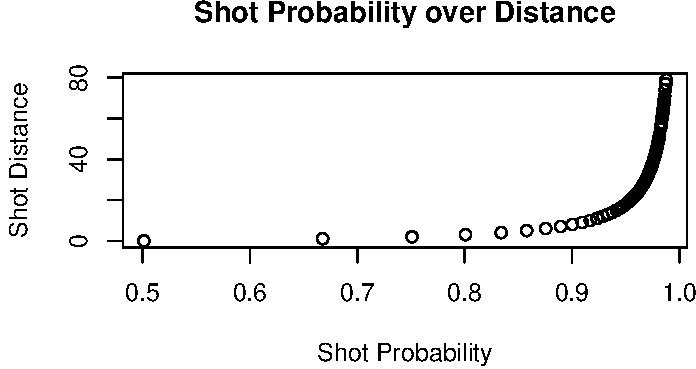
\includegraphics{Final_Project_Applied_files/figure-latex/Probabilities-1} \end{center}

\hypertarget{conclusion}{%
\section{\texorpdfstring{\textbf{Conclusion}}{Conclusion}}\label{conclusion}}

Analysis of the Kobe Bryant Shot Made data shows Kobe is consistent with his shot made by type, location on the court, distance from the hoop and whether he played a regular season game or a playoff game. Based on the analysis performed, a Logistic Regression Model produced better results than a Quadratic Discriminant Model after taking all variable and model analysis into consideration. These statistics are represented in Kobe Bryant's 20-year successful career.

\newpage

\hypertarget{appendix-a-figures-and-tables}{%
\section{Appendix A: Figures and Tables}\label{appendix-a-figures-and-tables}}

\hypertarget{appendix-a-contains-content-related-to-the-paper}{%
\subsubsection{\texorpdfstring{\emph{Appendix A contains content related to the paper}}{Appendix A contains content related to the paper}}\label{appendix-a-contains-content-related-to-the-paper}}

\hypertarget{receiver-operator-characteristic-roc-curves}{%
\subsection{\texorpdfstring{\textbf{Receiver Operator Characteristic (ROC) Curves}}{Receiver Operator Characteristic (ROC) Curves}}\label{receiver-operator-characteristic-roc-curves}}

\begin{center}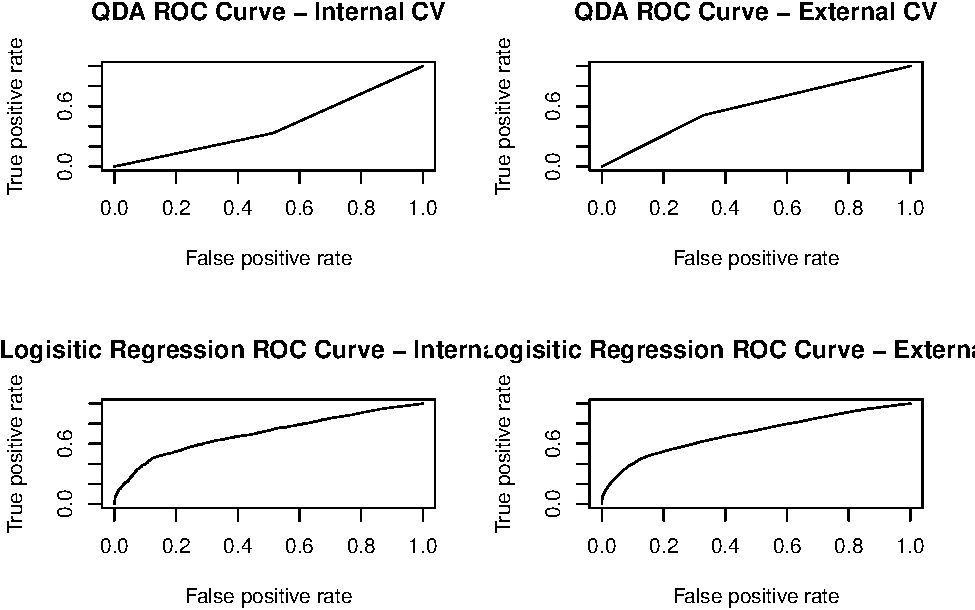
\includegraphics{Final_Project_Applied_files/figure-latex/ROC curves-1} \end{center}

\hypertarget{fitted-logistic-regression-model}{%
\subsection{\texorpdfstring{\textbf{Fitted Logistic Regression Model}}{Fitted Logistic Regression Model}}\label{fitted-logistic-regression-model}}

\begingroup\fontsize{10}{12}\selectfont

\begin{longtable}{lrr}
\toprule
  & Coefficient (logit) & Odds Ratio\\
\midrule
\endfirsthead
\multicolumn{3}{@{}l}{\textit{(continued)}}\\
\toprule
  & Coefficient (logit) & Odds Ratio\\
\midrule
\endhead
\
\endfoot
\bottomrule
\endlastfoot
\rowcolor{gray!6}  (Intercept) & 13.4225434 & 675050.9017498\\
recId & 0.0136368 & 1.0137302\\
\rowcolor{gray!6}  `action\_typeAlley Oop Layup shot` & -2.3205263 & 0.0982219\\
`action\_typeCutting Layup Shot` & -1.6513466 & 0.1917915\\
\rowcolor{gray!6}  `action\_typeDriving Bank shot` & 10.5208422 & 37080.3407836\\
\addlinespace
`action\_typeDriving Dunk Shot` & 0.5245757 & 1.6897417\\
\rowcolor{gray!6}  `action\_typeDriving Finger Roll Layup Shot` & -1.1149420 & 0.3279343\\
`action\_typeDriving Finger Roll Shot` & -1.8462292 & 0.1578312\\
\rowcolor{gray!6}  `action\_typeDriving Floating Bank Jump Shot` & 10.1961843 & 26800.7262599\\
`action\_typeDriving Floating Jump Shot` & -3.4111350 & 0.0330037\\
\addlinespace
\rowcolor{gray!6}  `action\_typeDriving Hook Shot` & -2.7840394 & 0.0617884\\
`action\_typeDriving Jump shot` & -4.0797951 & 0.0169109\\
\rowcolor{gray!6}  `action\_typeDriving Layup Shot` & -2.2080771 & 0.1099118\\
`action\_typeDriving Reverse Layup Shot` & -1.9126942 & 0.1476820\\
\rowcolor{gray!6}  `action\_typeDriving Slam Dunk Shot` & 0.1321462 & 1.1412751\\
\addlinespace
`action\_typeDunk Shot` & -2.2672636 & 0.1035953\\
\rowcolor{gray!6}  `action\_typeFadeaway Bank shot` & -0.7136965 & 0.4898302\\
`action\_typeFadeaway Jump Shot` & -3.0468033 & 0.0475106\\
\rowcolor{gray!6}  `action\_typeFinger Roll Layup Shot` & -2.3265883 & 0.0976283\\
`action\_typeFinger Roll Shot` & -3.1228802 & 0.0440302\\
\addlinespace
\rowcolor{gray!6}  `action\_typeFloating Jump shot` & -2.2637304 & 0.1039619\\
`action\_typeFollow Up Dunk Shot` & -1.0661569 & 0.3443293\\
\rowcolor{gray!6}  `action\_typeHook Bank Shot` & 10.2134549 & 27267.6128041\\
`action\_typeHook Shot` & -3.8692331 & 0.0208744\\
\rowcolor{gray!6}  `action\_typeJump Bank Shot` & -2.0944755 & 0.1231348\\
\addlinespace
`action\_typeJump Hook Shot` & -2.0526109 & 0.1283992\\
\rowcolor{gray!6}  `action\_typeJump Shot` & -4.1200063 & 0.0162444\\
`action\_typeLayup Shot` & -3.8516668 & 0.0212443\\
\rowcolor{gray!6}  `action\_typePullup Bank shot` & -2.9546883 & 0.0520949\\
`action\_typePullup Jump shot` & -2.2243604 & 0.1081366\\
\addlinespace
\rowcolor{gray!6}  `action\_typePutback Dunk Shot` & -2.7899501 & 0.0614243\\
`action\_typePutback Layup Shot` & -2.6921832 & 0.0677329\\
\rowcolor{gray!6}  `action\_typeReverse Dunk Shot` & 0.0771918 & 1.0802493\\
`action\_typeReverse Layup Shot` & -2.8497340 & 0.0578597\\
\rowcolor{gray!6}  `action\_typeReverse Slam Dunk Shot` & 10.2986570 & 29692.7136466\\
\addlinespace
`action\_typeRunning Bank shot` & -1.5553045 & 0.2111251\\
\rowcolor{gray!6}  `action\_typeRunning Dunk Shot` & -1.5628760 & 0.2095326\\
`action\_typeRunning Finger Roll Layup Shot` & -2.8121239 & 0.0600773\\
\rowcolor{gray!6}  `action\_typeRunning Finger Roll Shot` & -16.9093575 & 0.0000000\\
`action\_typeRunning Hook Shot` & -1.8963490 & 0.1501157\\
\addlinespace
\rowcolor{gray!6}  `action\_typeRunning Jump Shot` & -2.2497152 & 0.1054292\\
`action\_typeRunning Layup Shot` & -2.8535071 & 0.0576418\\
\rowcolor{gray!6}  `action\_typeRunning Pull-Up Jump Shot` & -16.5617800 & 0.0000001\\
`action\_typeRunning Reverse Layup Shot` & -4.5986325 & 0.0100656\\
\rowcolor{gray!6}  `action\_typeSlam Dunk Shot` & 0.8467543 & 2.3320653\\
\addlinespace
`action\_typeStep Back Jump shot` & -2.5585379 & 0.0774179\\
\rowcolor{gray!6}  `action\_typeTip Shot` & -4.1454923 & 0.0158356\\
`action\_typeTurnaround Bank shot` & -1.9936634 & 0.1361956\\
\rowcolor{gray!6}  `action\_typeTurnaround Fadeaway shot` & -3.0459246 & 0.0475523\\
`action\_typeTurnaround Finger Roll Shot` & 9.9543965 & 21044.5414151\\
\addlinespace
\rowcolor{gray!6}  `action\_typeTurnaround Hook Shot` & -3.4711028 & 0.0310827\\
`action\_typeTurnaround Jump Shot` & -2.9466004 & 0.0525179\\
\rowcolor{gray!6}  game\_event\_id & -0.0002398 & 0.9997602\\
loc\_x & 0.0001497 & 1.0001498\\
\rowcolor{gray!6}  minutes\_remaining & 0.0122044 & 1.0122792\\
\addlinespace
`season1997-98` & -0.0578076 & 0.9438315\\
\rowcolor{gray!6}  `season1998-99` & 0.3796978 & 1.4618428\\
`season1999-00` & 0.5389535 & 1.7142120\\
\rowcolor{gray!6}  `season2000-01` & 0.7859562 & 2.1945043\\
`season2001-02` & 0.8929332 & 2.4422828\\
\addlinespace
\rowcolor{gray!6}  `season2002-03` & 0.9829625 & 2.6723614\\
`season2003-04` & 0.9639388 & 2.6220037\\
\rowcolor{gray!6}  `season2004-05` & 1.4038822 & 4.0709735\\
`season2005-06` & 1.6091042 & 4.9983318\\
\rowcolor{gray!6}  `season2006-07` & 1.7103964 & 5.5311536\\
\addlinespace
`season2007-08` & 1.7773374 & 5.9140887\\
\rowcolor{gray!6}  `season2008-09` & 2.0093797 & 7.4586889\\
`season2009-10` & 1.9749527 & 7.2062790\\
\rowcolor{gray!6}  `season2010-11` & 2.1296754 & 8.4121361\\
`season2011-12` & 2.2033561 & 9.0553535\\
\addlinespace
\rowcolor{gray!6}  `season2012-13` & 2.4169619 & 11.2117448\\
`season2013-14` & 1.6501936 & 5.2079882\\
\rowcolor{gray!6}  `season2014-15` & 2.4556923 & 11.6544994\\
`season2015-16` & 2.5550064 & 12.8713824\\
\rowcolor{gray!6}  seconds\_remaining & 0.0025664 & 1.0025697\\
\addlinespace
shot\_distance & 0.0053921 & 1.0054066\\
\rowcolor{gray!6}  game\_date & -0.0004337 & 0.9995664\\
shot\_id & -0.0136309 & 0.9864616\\
\rowcolor{gray!6}  attendance & 0.0001672 & 1.0001673\\
arena\_temp & 0.0374076 & 1.0381160\\
\addlinespace
\rowcolor{gray!6}  playoffs & -0.0373788 & 0.9633111\\*
\end{longtable}
\endgroup{}

\hypertarget{action-type-frequency-table}{%
\subsection{\texorpdfstring{\textbf{Action Type Frequency Table}}{Action Type Frequency Table}}\label{action-type-frequency-table}}

\begingroup\fontsize{10}{12}\selectfont

\begin{longtable}{lr}
\toprule
Var1 & Freq\\
\midrule
\endfirsthead
\multicolumn{2}{@{}l}{\textit{(continued)}}\\
\toprule
Var1 & Freq\\
\midrule
\endhead
\
\endfoot
\bottomrule
\endlastfoot
\rowcolor{gray!6}  Alley Oop Dunk Shot & 76\\
Alley Oop Layup shot & 59\\
\rowcolor{gray!6}  Cutting Layup Shot & 6\\
Driving Bank shot & 1\\
\rowcolor{gray!6}  Driving Dunk Shot & 196\\
\addlinespace
Driving Finger Roll Layup Shot & 47\\
\rowcolor{gray!6}  Driving Finger Roll Shot & 52\\
Driving Floating Bank Jump Shot & 1\\
\rowcolor{gray!6}  Driving Floating Jump Shot & 3\\
Driving Hook Shot & 13\\
\addlinespace
\rowcolor{gray!6}  Driving Jump shot & 19\\
Driving Layup Shot & 1335\\
\rowcolor{gray!6}  Driving Reverse Layup Shot & 67\\
Driving Slam Dunk Shot & 38\\
\rowcolor{gray!6}  Dunk Shot & 176\\
\addlinespace
Fadeaway Bank shot & 22\\
\rowcolor{gray!6}  Fadeaway Jump Shot & 693\\
Finger Roll Layup Shot & 21\\
\rowcolor{gray!6}  Finger Roll Shot & 23\\
Floating Jump shot & 75\\
\addlinespace
\rowcolor{gray!6}  Follow Up Dunk Shot & 10\\
Hook Bank Shot & 5\\
\rowcolor{gray!6}  Hook Shot & 61\\
Jump Bank Shot & 223\\
\rowcolor{gray!6}  Jump Hook Shot & 16\\
\addlinespace
Jump Shot & 12712\\
\rowcolor{gray!6}  Layup Shot & 1734\\
Pullup Bank shot & 10\\
\rowcolor{gray!6}  Pullup Jump shot & 318\\
Putback Dunk Shot & 3\\
\addlinespace
\rowcolor{gray!6}  Putback Layup Shot & 9\\
Reverse Dunk Shot & 52\\
\rowcolor{gray!6}  Reverse Layup Shot & 276\\
Reverse Slam Dunk Shot & 15\\
\rowcolor{gray!6}  Running Bank shot & 35\\
\addlinespace
Running Dunk Shot & 14\\
\rowcolor{gray!6}  Running Finger Roll Layup Shot & 5\\
Running Finger Roll Shot & 4\\
\rowcolor{gray!6}  Running Hook Shot & 28\\
Running Jump Shot & 620\\
\addlinespace
\rowcolor{gray!6}  Running Layup Shot & 42\\
Running Pull-Up Jump Shot & 1\\
\rowcolor{gray!6}  Running Reverse Layup Shot & 6\\
Slam Dunk Shot & 264\\
\rowcolor{gray!6}  Step Back Jump shot & 93\\
\addlinespace
Tip Shot & 121\\
\rowcolor{gray!6}  Turnaround Bank shot & 50\\
Turnaround Fadeaway shot & 299\\
\rowcolor{gray!6}  Turnaround Finger Roll Shot & 1\\
Turnaround Hook Shot & 8\\
\addlinespace
\rowcolor{gray!6}  Turnaround Jump Shot & 739\\*
\end{longtable}
\endgroup{}

\hypertarget{variance-inflation-factor}{%
\subsection{\texorpdfstring{\textbf{Variance Inflation Factor}}{Variance Inflation Factor}}\label{variance-inflation-factor}}

\begin{table}[H]
\centering
\begin{tabular}{lr}
\toprule
Variable & Variance Inflation Factor\\
\midrule
\rowcolor{gray!6}  shot\_id & 41103299.94\\
recId & 41101644.14\\
\rowcolor{gray!6}  shot\_distance & 3.75\\
loc\_y & 3.31\\
\rowcolor{gray!6}  shot\_type & 1.88\\
\addlinespace
playoffs & 1.78\\
\rowcolor{gray!6}  game\_event\_id & 1.60\\
attendance & 1.39\\
\rowcolor{gray!6}  avgnoisedb & 1.37\\
game\_date & 1.15\\
\addlinespace
\rowcolor{gray!6}  minutes\_remaining & 1.09\\
shot\_made\_flag & 1.06\\
\rowcolor{gray!6}  arena\_temp & 1.02\\
seconds\_remaining & 1.01\\
\rowcolor{gray!6}  loc\_x & 1.01\\
\bottomrule
\end{tabular}
\end{table}

\newpage

\hypertarget{appendix-b-source-code}{%
\section{Appendix B: Source Code}\label{appendix-b-source-code}}

\hypertarget{appendix-a-contains-source-code-created-for-this-project}{%
\subsubsection{\texorpdfstring{\emph{Appendix A contains source code created for this project}}{Appendix A contains source code created for this project}}\label{appendix-a-contains-source-code-created-for-this-project}}

\hypertarget{loading-libraries-importing-data}{%
\subsection{Loading Libraries, Importing Data}\label{loading-libraries-importing-data}}

\begin{Shaded}
\begin{Highlighting}[]


\KeywordTok{library}\NormalTok{(pacman)}
\KeywordTok{p_load}\NormalTok{(rrcov, MASS, dplyr, purrr, ggplot2, Hmisc, pcaPP, knitr, kableExtra, caret, }
\NormalTok{cluster, robustbase, ROCR, Metrics, bookdown, ResourceSelection, usdm)}

\CommentTok{# Reading Data}
\NormalTok{df <-}\StringTok{ }\KeywordTok{read.csv}\NormalTok{(}\StringTok{"./modelingKobeData.csv"}\NormalTok{, }\DataTypeTok{header=}\NormalTok{T, }\DataTypeTok{sep=}\StringTok{","}\NormalTok{, }\DataTypeTok{strip.white=}\NormalTok{T, }
\DataTypeTok{stringsAsFactors =}\NormalTok{ F, }\DataTypeTok{na.strings=}\KeywordTok{c}\NormalTok{(}\StringTok{""}\NormalTok{))}
\NormalTok{df.preds <-}\StringTok{ }\KeywordTok{read.csv}\NormalTok{(}\StringTok{"./predictionKobeData.csv"}\NormalTok{, }\DataTypeTok{header=}\NormalTok{T, }\DataTypeTok{sep=}\StringTok{","}\NormalTok{, }
\DataTypeTok{strip.white=}\NormalTok{T, }\DataTypeTok{stringsAsFactors =}\NormalTok{ F, }\DataTypeTok{na.strings=}\KeywordTok{c}\NormalTok{(}\StringTok{""}\NormalTok{))}
\end{Highlighting}
\end{Shaded}

\hypertarget{check-for-missing-values}{%
\subsection{Check for Missing Values}\label{check-for-missing-values}}

\begin{Shaded}
\begin{Highlighting}[]
\KeywordTok{sapply}\NormalTok{(df, }\ControlFlowTok{function}\NormalTok{(cnt) }\KeywordTok{sum}\NormalTok{(}\KeywordTok{length}\NormalTok{(}\KeywordTok{which}\NormalTok{(}\KeywordTok{is.na}\NormalTok{(cnt)))))}
\end{Highlighting}
\end{Shaded}

\hypertarget{basketball-shot-location-map}{%
\subsection{Basketball Shot Location Map}\label{basketball-shot-location-map}}

\begin{Shaded}
\begin{Highlighting}[]
\NormalTok{shotsTaken <-}\StringTok{ }\KeywordTok{data.frame}\NormalTok{(df}\OperatorTok{$}\NormalTok{loc_x, df}\OperatorTok{$}\NormalTok{loc_y, df}\OperatorTok{$}\NormalTok{shot_distance)}
\KeywordTok{colnames}\NormalTok{(shotsTaken) <-}\StringTok{ }\KeywordTok{c}\NormalTok{(}\StringTok{"loc_x"}\NormalTok{, }\StringTok{"loc_y"}\NormalTok{, }\StringTok{"shot_distance"}\NormalTok{)}


\KeywordTok{ggplot}\NormalTok{(shotsTaken, }\KeywordTok{aes}\NormalTok{(}\DataTypeTok{x=}\NormalTok{loc_x, }\DataTypeTok{y=}\NormalTok{loc_y)) }\OperatorTok{+}\StringTok{ }
\StringTok{  }\KeywordTok{geom_point}\NormalTok{(}\KeywordTok{aes}\NormalTok{(}\DataTypeTok{colour =}\NormalTok{ df}\OperatorTok{$}\NormalTok{shot_type))}
\end{Highlighting}
\end{Shaded}

\hypertarget{shot-location-imputing-toint-conversion}{%
\subsection{Shot Location Imputing, toInt Conversion}\label{shot-location-imputing-toint-conversion}}

\begin{Shaded}
\begin{Highlighting}[]
\NormalTok{df[}\KeywordTok{which}\NormalTok{(df}\OperatorTok{$}\NormalTok{loc_y }\OperatorTok{>}\StringTok{ }\DecValTok{300}\NormalTok{),}\StringTok{"shot_type"}\NormalTok{] <-}\StringTok{ "3PT Field Goal"}
\NormalTok{df.preds[}\KeywordTok{which}\NormalTok{(df.preds}\OperatorTok{$}\NormalTok{loc_y }\OperatorTok{>}\StringTok{ }\DecValTok{300}\NormalTok{),}\StringTok{"shot_type"}\NormalTok{] <-}\StringTok{ "3PT Field Goal"}

\CommentTok{# Convert the points to integer values}
\NormalTok{df}\OperatorTok{$}\NormalTok{shot_type <-}\StringTok{ }\KeywordTok{ifelse}\NormalTok{(df}\OperatorTok{$}\NormalTok{shot_type}\OperatorTok{==}\StringTok{"2PT Field Goal"}\NormalTok{, }\DecValTok{2}\NormalTok{, }\DecValTok{3}\NormalTok{)}
\NormalTok{df.preds}\OperatorTok{$}\NormalTok{shot_type <-}\StringTok{ }\KeywordTok{ifelse}\NormalTok{(df.preds}\OperatorTok{$}\NormalTok{shot_type}\OperatorTok{==}\StringTok{"2PT Field Goal"}\NormalTok{, }\DecValTok{2}\NormalTok{, }\DecValTok{3}\NormalTok{)}
\end{Highlighting}
\end{Shaded}

\hypertarget{variable-eliminations-first-pass}{%
\subsection{Variable Eliminations, First-Pass}\label{variable-eliminations-first-pass}}

\begin{Shaded}
\begin{Highlighting}[]

\NormalTok{df <-}\StringTok{ }\NormalTok{df }\OperatorTok\StringTok{ }\KeywordTok{mutate_if}\NormalTok{(is.integer, as.numeric) }\OperatorTok\StringTok{ }
\KeywordTok{mutate_if}\NormalTok{(is.character, as.factor) }\OperatorTok\StringTok{ }\KeywordTok{data.frame}\NormalTok{()}
\NormalTok{df <-}\StringTok{ }\NormalTok{df }\OperatorTok\StringTok{ }
\StringTok{        }\KeywordTok{subset}\NormalTok{(}\DataTypeTok{select=}\OperatorTok{-}\KeywordTok{c}\NormalTok{(}
\NormalTok{team_id, }\CommentTok{# dropping since this is a uniform distribution of data}
\NormalTok{team_name, }\CommentTok{# dropping since this is a uniform distribution of data. Also }
\NormalTok{collinear with team_id}
\NormalTok{combined_shot_type, }\CommentTok{# dropping this in favor of combined_shot_type}
\NormalTok{shot_zone_area, }\CommentTok{# this is ambiguous and less descriptive than geospatial data}
\NormalTok{shot_zone_range,}
\NormalTok{shot_zone_basic,}
\NormalTok{matchup }\CommentTok{# removing in favor of opponent; Kobe only played for LAL so that }
\NormalTok{will never change}
\NormalTok{        )}
\NormalTok{)}

\NormalTok{df.preds <-}\StringTok{ }\NormalTok{df.preds }\OperatorTok\StringTok{ }
\KeywordTok{mutate_if}\NormalTok{(is.integer, as.numeric) }\OperatorTok\StringTok{ }\KeywordTok{mutate_if}\NormalTok{(is.character, as.factor) }\OperatorTok\StringTok{ }
\KeywordTok{data.frame}\NormalTok{()}
\NormalTok{df.preds <-}\StringTok{ }\NormalTok{df.preds }\OperatorTok\StringTok{ }
\StringTok{  }\KeywordTok{subset}\NormalTok{(}\DataTypeTok{select=}\OperatorTok{-}\KeywordTok{c}\NormalTok{(}
\NormalTok{  team_id, }\CommentTok{# dropping since this is a uniform distribution of data}
\NormalTok{  team_name, }\CommentTok{# dropping since this is a uniform distribution of data. Also }
\NormalTok{  collinear with team_id}
\NormalTok{  combined_shot_type, }\CommentTok{# dropping this in favor of combined_shot_type}
\NormalTok{  shot_zone_area, }\CommentTok{# this is ambiguous and less descriptive than geospatial data}
\NormalTok{  shot_zone_range,}
\NormalTok{  shot_zone_basic,}
\NormalTok{  matchup }\CommentTok{# removing in favor of opponent; Kobe only played for LAL so that }
\NormalTok{  will never change}
\NormalTok{                  )}
\NormalTok{          )}

\CommentTok{# create numeric dataframe for correlation plot}
\NormalTok{df.numeric <-}\StringTok{ }\NormalTok{df }\OperatorTok\StringTok{ }\KeywordTok{keep}\NormalTok{(is.numeric)}
\NormalTok{df.numeric.preds <-}\StringTok{ }\NormalTok{df.preds }\OperatorTok\StringTok{ }\KeywordTok{keep}\NormalTok{(is.numeric)}
\end{Highlighting}
\end{Shaded}

\hypertarget{correlation-heat-map}{%
\subsection{Correlation Heat Map}\label{correlation-heat-map}}

\begin{Shaded}
\begin{Highlighting}[]
\NormalTok{corr.plot <-}\StringTok{ }\NormalTok{corrplot}\OperatorTok{::}\KeywordTok{corrplot}\NormalTok{(}\KeywordTok{cor}\NormalTok{(df.numeric }\OperatorTok\StringTok{ }\KeywordTok{subset}\NormalTok{(}\DataTypeTok{select=}\OperatorTok{-}\KeywordTok{c}\NormalTok{(}
\NormalTok{shot_made_flag)))}
\NormalTok{                   , }\DataTypeTok{title =} \StringTok{"Correlation among Predictor Variables"}
\NormalTok{                   , }\DataTypeTok{type =} \StringTok{"lower"}
\NormalTok{                   , }\DataTypeTok{tl.pos =} \StringTok{"ld"}
\NormalTok{                   , }\DataTypeTok{method =} \StringTok{"square"}
\NormalTok{                   , }\DataTypeTok{tl.cex =} \FloatTok{0.65}
\NormalTok{                   , }\DataTypeTok{tl.col =} \StringTok{'red'}
\NormalTok{                   , }\DataTypeTok{order =} \StringTok{"alphabet"}
\NormalTok{                   , }\DataTypeTok{diag =}\NormalTok{ F}
\NormalTok{                   , }\DataTypeTok{mar=}\KeywordTok{c}\NormalTok{(}\DecValTok{0}\NormalTok{,}\DecValTok{0}\NormalTok{,}\DecValTok{5}\NormalTok{,}\DecValTok{0}\NormalTok{)}
\NormalTok{                   , }\DataTypeTok{bg=}\StringTok{"ivory1"}
\NormalTok{                   ,}\DataTypeTok{tl.srt=}\NormalTok{.}\DecValTok{05}
\NormalTok{)}
\end{Highlighting}
\end{Shaded}

\hypertarget{variance-inflation-factor-table}{%
\subsection{Variance Inflation Factor Table}\label{variance-inflation-factor-table}}

\begin{Shaded}
\begin{Highlighting}[]
\NormalTok{vifFrame <-}\StringTok{ }\KeywordTok{vif}\NormalTok{(df.numeric)}
\NormalTok{vifFrame <-}\StringTok{ }\NormalTok{vifFrame[}\KeywordTok{order}\NormalTok{(}\OperatorTok{-}\NormalTok{vifFrame}\OperatorTok{$}\NormalTok{VIF),]}
\NormalTok{vifFrame.Top7 <-}\StringTok{ }\KeywordTok{data.frame}\NormalTok{(}\KeywordTok{head}\NormalTok{(vifFrame, }\DecValTok{7}\NormalTok{))}
\end{Highlighting}
\end{Shaded}

\hypertarget{variable-eliminations-second-pass}{%
\subsection{Variable Eliminations, Second Pass}\label{variable-eliminations-second-pass}}

\begin{Shaded}
\begin{Highlighting}[]

\NormalTok{df <-}\StringTok{ }\NormalTok{df }\OperatorTok\StringTok{ }\KeywordTok{subset}\NormalTok{(}\DataTypeTok{select=}\OperatorTok{-}\KeywordTok{c}\NormalTok{(}
\NormalTok{  lat, }\CommentTok{# dropping lat because it is collinear with loc_y and shot_distance}
\NormalTok{  lon, }\CommentTok{# dropping lon because it is collinear with loc_x and shot_distance}
\NormalTok{  period, }\CommentTok{# dropping period in favor of game event id - game event id is }
          \CommentTok{# more descriptive and continuous}
\NormalTok{  game_id }\CommentTok{# dropping playoffs for game_id; }
          \CommentTok{# game ID can capture playoffs seasonally}
\NormalTok{                             )}
\NormalTok{                    )}

\NormalTok{df.preds <-}\StringTok{ }\NormalTok{df.preds }\OperatorTok\StringTok{ }\KeywordTok{subset}\NormalTok{(}\DataTypeTok{select=}\OperatorTok{-}\KeywordTok{c}\NormalTok{(}
\NormalTok{  lat,}
\NormalTok{  lon,}
\NormalTok{  period,}
\NormalTok{  game_id}
\NormalTok{                             )}
\NormalTok{                    )}

\NormalTok{df.numeric <-}\StringTok{ }\NormalTok{df }\OperatorTok\StringTok{ }\KeywordTok{keep}\NormalTok{(is.numeric) }\OperatorTok\StringTok{ }\KeywordTok{mutate_if}\NormalTok{(is.integer, as.numeric)}
\NormalTok{df.numeric.preds <-}\StringTok{ }\NormalTok{df.preds }\OperatorTok\StringTok{ }\KeywordTok{keep}\NormalTok{(is.numeric) }\OperatorTok\StringTok{ }\KeywordTok{mutate_if}\NormalTok{(}
\NormalTok{is.integer, as.numeric)}
\end{Highlighting}
\end{Shaded}

\hypertarget{correlation-matrix}{%
\subsection{Correlation Matrix}\label{correlation-matrix}}

\begin{Shaded}
\begin{Highlighting}[]
\NormalTok{flattenCorrMatrix <-}\StringTok{ }\ControlFlowTok{function}\NormalTok{(cormatrix, pmatrix) \{}
\NormalTok{  ut <-}\StringTok{ }\KeywordTok{upper.tri}\NormalTok{(cormatrix)}
  \KeywordTok{data.frame}\NormalTok{(}
    \DataTypeTok{row =} \KeywordTok{rownames}\NormalTok{(cormatrix)[}\KeywordTok{row}\NormalTok{(cormatrix)[ut]],}
    \DataTypeTok{column =} \KeywordTok{rownames}\NormalTok{(cormatrix)[}\KeywordTok{col}\NormalTok{(cormatrix)[ut]],}
    \DataTypeTok{cor  =}\NormalTok{(cormatrix)[ut],}
    \DataTypeTok{p =}\NormalTok{ pmatrix[ut]}
\NormalTok{  )}
\NormalTok{\}}

\KeywordTok{options}\NormalTok{(}\DataTypeTok{scipen=}\DecValTok{999}\NormalTok{)}
\KeywordTok{options}\NormalTok{(}\DataTypeTok{max.print=}\DecValTok{100000}\NormalTok{)}

\NormalTok{correlation.matrix <-}\StringTok{ }\NormalTok{Hmisc}\OperatorTok{::}\KeywordTok{rcorr}\NormalTok{(}\KeywordTok{as.matrix}\NormalTok{(df.numeric), }\DataTypeTok{type=}\StringTok{"pearson"}\NormalTok{)}
\NormalTok{corDF <-}\StringTok{ }\KeywordTok{data.frame}\NormalTok{(}\KeywordTok{flattenCorrMatrix}\NormalTok{(correlation.matrix}\OperatorTok{$}\NormalTok{r, }
\NormalTok{correlation.matrix}\OperatorTok{$}\NormalTok{P))}

\NormalTok{corDF.ordered <-}\StringTok{ }\KeywordTok{data.frame}\NormalTok{(corDF[}\KeywordTok{order}\NormalTok{(}\OperatorTok{-}\NormalTok{corDF}\OperatorTok{$}\NormalTok{cor),])}
\NormalTok{cordDF.ordered.Top10 <-}\StringTok{ }\KeywordTok{data.frame}\NormalTok{(}\KeywordTok{head}\NormalTok{(corDF.ordered, }\DecValTok{10}\NormalTok{), }\DataTypeTok{row.names =}\NormalTok{ F)}

\KeywordTok{colnames}\NormalTok{(cordDF.ordered.Top10) =}\StringTok{ }\KeywordTok{c}\NormalTok{(}\StringTok{"Correlation Predictor Variable"}\NormalTok{, }
\StringTok{"Correlation Response Variable"}\NormalTok{, }\StringTok{"Correlation"}\NormalTok{, }\StringTok{"p-Value"}\NormalTok{)}

\NormalTok{cordDF.ordered.Top10}\OperatorTok{$}\NormalTok{Correlation <-}\StringTok{ }\KeywordTok{round}\NormalTok{(}\KeywordTok{as.numeric}\NormalTok{(}\KeywordTok{as.character}\NormalTok{(}
\NormalTok{cordDF.ordered.Top10}\OperatorTok{$}\NormalTok{Correlation)), }\DataTypeTok{digits=}\DecValTok{5}\NormalTok{)}

\NormalTok{cordDF.ordered.Top10}\OperatorTok{$}\StringTok{`}\DataTypeTok{p-Value}\StringTok{`}\NormalTok{ <-}\StringTok{ }\KeywordTok{ifelse}\NormalTok{(}\KeywordTok{as.numeric}\NormalTok{(}\KeywordTok{as.character}\NormalTok{(}
\NormalTok{cordDF.ordered.Top10}\OperatorTok{$}\StringTok{`}\DataTypeTok{p-Value}\StringTok{`}\NormalTok{)) }\OperatorTok{<}\StringTok{ }\FloatTok{0.0001}\NormalTok{, }\StringTok{"p < 0.0001"}\NormalTok{, }\KeywordTok{as.numeric}\NormalTok{(}\KeywordTok{as.character}\NormalTok{(}
\NormalTok{cordDF.ordered.Top10}\OperatorTok{$}\StringTok{`}\DataTypeTok{p-Value}\StringTok{`}\NormalTok{)))}
\end{Highlighting}
\end{Shaded}

\hypertarget{qda-bartlett-approximation}{%
\subsection{QDA Bartlett Approximation}\label{qda-bartlett-approximation}}

\begin{Shaded}
\begin{Highlighting}[]

\NormalTok{dfTrain.numeric <-}\StringTok{ }\NormalTok{df.numeric[}\KeywordTok{which}\NormalTok{(}\OperatorTok{!}\KeywordTok{is.na}\NormalTok{(df.numeric}\OperatorTok{$}\NormalTok{shot_made_flag)),]}
\NormalTok{prediction.Data.numeric <-}\StringTok{ }\NormalTok{df.numeric[}\KeywordTok{which}\NormalTok{(}\KeywordTok{is.na}\NormalTok{(df.numeric}\OperatorTok{$}\NormalTok{shot_made_flag)),]}

\NormalTok{dfTrain.numeric}\OperatorTok{$}\NormalTok{shot_made_flag <-}\StringTok{ }\KeywordTok{as.factor}\NormalTok{(dfTrain.numeric}\OperatorTok{$}\NormalTok{shot_made_flag)}
\NormalTok{dfTrain.numeric}\OperatorTok{$}\NormalTok{shot_made_flag <-}\StringTok{ }\KeywordTok{ifelse}\NormalTok{(dfTrain.numeric}\OperatorTok{$}\NormalTok{shot_made_flag}\OperatorTok{==}\StringTok{"1"}\NormalTok{, }
\StringTok{"made"}\NormalTok{, }\StringTok{"not_made"}\NormalTok{)}
\NormalTok{dfTrain.numeric <-}\StringTok{ }\NormalTok{dfTrain.numeric }\OperatorTok\StringTok{ }\KeywordTok{mutate_if}\NormalTok{(is.integer, as.numeric) }\OperatorTok\StringTok{ }
\KeywordTok{mutate_if}\NormalTok{(is.character, as.factor) }\OperatorTok\StringTok{ }\KeywordTok{data.frame}\NormalTok{()}

\NormalTok{Bartlett_ChiSq <-}\StringTok{ }\NormalTok{rrcov}\OperatorTok{::}\KeywordTok{Wilks.test}\NormalTok{(shot_made_flag }\OperatorTok{~}\StringTok{ }\NormalTok{., }\DataTypeTok{data=}\NormalTok{dfTrain.numeric, }
\DataTypeTok{method =} \StringTok{"c"}\NormalTok{, }\DataTypeTok{approximation =} \StringTok{"Bartlett"}\NormalTok{)}

\CommentTok{# Wilk's Lambda produces significant p-value in Bartlett's test so we need to }
\NormalTok{use a Quadratic Discriminant Analysis instead of Linear}
\KeywordTok{format}\NormalTok{(}\KeywordTok{round}\NormalTok{(Bartlett_ChiSq}\OperatorTok{$}\NormalTok{p.value, }\DecValTok{2}\NormalTok{), }\DataTypeTok{nsmall=}\DecValTok{4}\NormalTok{)}

\CommentTok{# Wilks' Lambda plus degrees of freedom used in Bartlett's chi-squared test}
\NormalTok{WilksDegreesofFreedom <-}\StringTok{ }\KeywordTok{rbind}\NormalTok{(}\KeywordTok{as.numeric}\NormalTok{(}\KeywordTok{paste0}\NormalTok{(Bartlett_ChiSq}\OperatorTok{$}\NormalTok{parameter, }\DataTypeTok{sep =} \StringTok{" "}\NormalTok{)))}

\CommentTok{# p-value from Bartlett's test}
\NormalTok{Bartlett_ChiSq}\OperatorTok{$}\NormalTok{p.value}
\NormalTok{Bartletts_p <-}\StringTok{ }\KeywordTok{format}\NormalTok{(}\KeywordTok{round}\NormalTok{(}\KeywordTok{as.numeric}\NormalTok{(Bartlett_ChiSq}\OperatorTok{$}\NormalTok{p.value), }\DecValTok{2}\NormalTok{), }\DataTypeTok{nsmall=}\DecValTok{4}\NormalTok{)}

\CommentTok{# Because Bartlett's p-value is less than 0.0001 (indicated above), updating to }
\NormalTok{shorter form}\OperatorTok{:}
\NormalTok{Bartletts_p =}\StringTok{ }\KeywordTok{ifelse}\NormalTok{(Bartlett_ChiSq}\OperatorTok{$}\NormalTok{p.value }\OperatorTok{<}\StringTok{ }\FloatTok{0.0001}\NormalTok{, }\StringTok{"p < 0.0001"}\NormalTok{, }
\NormalTok{Bartlett_ChiSq}\OperatorTok{$}\NormalTok{p.value)}
\CommentTok{#Bartletts_p <- "p < 0.0001"}

\NormalTok{dfBartlett <-}\StringTok{ }\KeywordTok{data.frame}\NormalTok{(WilksDegreesofFreedom, Bartlett_ChiSq}\OperatorTok{$}\NormalTok{wilks, Bartletts_p)}
\KeywordTok{colnames}\NormalTok{(dfBartlett) <-}\StringTok{ }\KeywordTok{c}\NormalTok{(}\StringTok{"Chi-Square Statistic"}\NormalTok{, }\StringTok{"Degrees of Freedom"}\NormalTok{, }
\StringTok{"Wilks' Lambda"}\NormalTok{, }\StringTok{"p-Value"}\NormalTok{)}

\NormalTok{dfBartlett}\OperatorTok{$}\StringTok{`}\DataTypeTok{Chi-Square Statistic}\StringTok{`}\NormalTok{ <-}\StringTok{ }\KeywordTok{round}\NormalTok{(}\KeywordTok{as.numeric}\NormalTok{(}\KeywordTok{as.character}\NormalTok{(}
\NormalTok{dfBartlett}\OperatorTok{$}\StringTok{`}\DataTypeTok{Chi-Square Statistic}\StringTok{`}\NormalTok{)), }\DataTypeTok{digits=}\DecValTok{5}\NormalTok{)}
\NormalTok{dfBartlett}\OperatorTok{$}\StringTok{`}\DataTypeTok{Wilks' Lambda}\StringTok{`}\NormalTok{ <-}\StringTok{ }\KeywordTok{round}\NormalTok{(}\KeywordTok{as.numeric}\NormalTok{(}\KeywordTok{as.character}\NormalTok{(}
\NormalTok{dfBartlett}\OperatorTok{$}\StringTok{`}\DataTypeTok{Wilks' Lambda}\StringTok{`}\NormalTok{)), }\DataTypeTok{digits=}\DecValTok{5}\NormalTok{)}

\NormalTok{bartlettsTest <-}\StringTok{ }\KeywordTok{data.frame}\NormalTok{(}\KeywordTok{rbind}\NormalTok{(dfBartlett}\OperatorTok{$}\StringTok{`}\DataTypeTok{Chi-Square Statistic}\StringTok{`}\NormalTok{, }
\NormalTok{dfBartlett}\OperatorTok{$}\StringTok{`}\DataTypeTok{Degrees of Freedom}\StringTok{`}\NormalTok{,dfBartlett}\OperatorTok{$}\StringTok{`}\DataTypeTok{Wilks' Lambda}\StringTok{`}\NormalTok{,Bartletts_p))}
\KeywordTok{rownames}\NormalTok{(bartlettsTest) <-}\StringTok{ }\KeywordTok{c}\NormalTok{(}\StringTok{"Chi Square Statistic"}\NormalTok{,}\StringTok{"Degrees of Freedom"}\NormalTok{,}
\StringTok{"Wilks' Lambda"}\NormalTok{,}\StringTok{"p-Value"}\NormalTok{)}
\KeywordTok{colnames}\NormalTok{(bartlettsTest) <-}\StringTok{ "Statistics"}
\end{Highlighting}
\end{Shaded}

\hypertarget{partitioning-training-testing-data}{%
\subsection{Partitioning Training, Testing Data}\label{partitioning-training-testing-data}}

\begin{Shaded}
\begin{Highlighting}[]

\NormalTok{dfTrain <-}\StringTok{ }\NormalTok{df[}\KeywordTok{which}\NormalTok{(}\OperatorTok{!}\KeywordTok{is.na}\NormalTok{(df}\OperatorTok{$}\NormalTok{shot_made_flag)),]}
\NormalTok{prediction.Data <-}\StringTok{ }\NormalTok{df[}\KeywordTok{which}\NormalTok{(}\KeywordTok{is.na}\NormalTok{(df}\OperatorTok{$}\NormalTok{shot_made_flag)),]}

\CommentTok{### Full Data train/test split for Logistic}
\NormalTok{test_sample_size <-}\StringTok{ }\KeywordTok{floor}\NormalTok{(}\FloatTok{0.75} \OperatorTok{*}\StringTok{ }\KeywordTok{nrow}\NormalTok{(dfTrain))}
\KeywordTok{set.seed}\NormalTok{(}\DecValTok{123}\NormalTok{)}
\NormalTok{train_ind <-}\StringTok{ }\KeywordTok{sample}\NormalTok{(}\KeywordTok{seq_len}\NormalTok{(}\KeywordTok{nrow}\NormalTok{(dfTrain)), }\DataTypeTok{size =}\NormalTok{ test_sample_size)}
\NormalTok{subDF.Train <-}\StringTok{ }\NormalTok{dfTrain[train_ind, ] }\CommentTok{#75% training}
\NormalTok{subDF.Test <-}\StringTok{ }\NormalTok{dfTrain[}\OperatorTok{-}\NormalTok{train_ind, ] }\CommentTok{# 25% testing}

\CommentTok{#### Numeric Data train/test split for QDA}
\NormalTok{test_sample_size <-}\StringTok{ }\KeywordTok{floor}\NormalTok{(}\FloatTok{0.75} \OperatorTok{*}\StringTok{ }\KeywordTok{nrow}\NormalTok{(dfTrain.numeric))}
\KeywordTok{set.seed}\NormalTok{(}\DecValTok{123}\NormalTok{)}
\NormalTok{train_ind <-}\StringTok{ }\KeywordTok{sample}\NormalTok{(}\KeywordTok{seq_len}\NormalTok{(}\KeywordTok{nrow}\NormalTok{(dfTrain.numeric)), }\DataTypeTok{size =}\NormalTok{ test_sample_size)}
\NormalTok{subDF.Train.numeric <-}\StringTok{ }\NormalTok{dfTrain.numeric[train_ind, ] }\CommentTok{#75% training}
\NormalTok{subDF.Test.numeric <-}\StringTok{ }\NormalTok{dfTrain.numeric[}\OperatorTok{-}\NormalTok{train_ind, ] }\CommentTok{# 25% testing}
\end{Highlighting}
\end{Shaded}

\hypertarget{a-priori-analysis}{%
\subsection{a Priori Analysis}\label{a-priori-analysis}}

\begin{Shaded}
\begin{Highlighting}[]
\CommentTok{# MASS package used for qda()}
\CommentTok{#df.numeric <- df.numeric[order(df.numeric$shot_made_flag),]}
\NormalTok{kobe.qda <-}\StringTok{ }\KeywordTok{qda}\NormalTok{(shot_made_flag }\OperatorTok{~}\StringTok{ }\NormalTok{., }\DataTypeTok{CV=}\NormalTok{T, }\DataTypeTok{data=}\NormalTok{dfTrain.numeric)}

\KeywordTok{data.frame}\NormalTok{(}\KeywordTok{mean}\NormalTok{(kobe.qda}\OperatorTok{$}\NormalTok{posterior[,}\DecValTok{1}\NormalTok{]), }\KeywordTok{mean}\NormalTok{(kobe.qda}\OperatorTok{$}\NormalTok{posterior[,}\DecValTok{2}\NormalTok{]))}

\NormalTok{shot_made_flag_Posterior <-}\StringTok{ }\KeywordTok{rbind}\NormalTok{(}\StringTok{"0"}\NormalTok{, }\StringTok{"1"}\NormalTok{)}
\CommentTok{# a Priori noted, used for testing, but default for proportions used}
\NormalTok{proportion_Posterior <-}\StringTok{ }\KeywordTok{rbind}\NormalTok{(}\KeywordTok{mean}\NormalTok{(kobe.qda}\OperatorTok{$}\NormalTok{posterior[,}\DecValTok{1}\NormalTok{]), }\KeywordTok{mean}\NormalTok{(}
\NormalTok{kobe.qda}\OperatorTok{$}\NormalTok{posterior[,}\DecValTok{2}\NormalTok{]))}
\NormalTok{priori <-}\StringTok{ }\KeywordTok{data.frame}\NormalTok{(shot_made_flag_Posterior, proportion_Posterior)}
\end{Highlighting}
\end{Shaded}

\hypertarget{quadratic-discriminant-analysis-internal-cv-and-model-development}{%
\subsection{Quadratic Discriminant Analysis: Internal CV and Model Development}\label{quadratic-discriminant-analysis-internal-cv-and-model-development}}

\begin{Shaded}
\begin{Highlighting}[]

\NormalTok{subDF.Train.numeric}\OperatorTok{$}\NormalTok{shot_made_flag <-}\StringTok{ }\KeywordTok{as.factor}\NormalTok{(}
\NormalTok{subDF.Train.numeric}\OperatorTok{$}\NormalTok{shot_made_flag)}
\CommentTok{#subDF.Train.numeric$shot_made_flag <- ifelse(}
\NormalTok{subDF.Train.numeric}\OperatorTok{$}\NormalTok{shot_made_flag}\OperatorTok{==}\StringTok{"1"}\NormalTok{, }\StringTok{"made"}\NormalTok{, }\StringTok{"not_made"}\ErrorTok{)}
\NormalTok{subDF.Train.numeric <-}\StringTok{ }\NormalTok{subDF.Train.numeric }\OperatorTok\StringTok{ }\KeywordTok{mutate_if}\NormalTok{(}
\NormalTok{is.integer, as.numeric) }\OperatorTok\StringTok{ }\KeywordTok{mutate_if}\NormalTok{(is.character, as.factor) }\OperatorTok\StringTok{ }
\KeywordTok{data.frame}\NormalTok{()}

\CommentTok{# k=25 folds, repeat random folding for internal cross-validation 5 times:}
\NormalTok{train.Control <-}\StringTok{ }\NormalTok{caret}\OperatorTok{::}\KeywordTok{trainControl}\NormalTok{(}\DataTypeTok{method =} \StringTok{"repeatedcv"}\NormalTok{,}
                              \DataTypeTok{number =} \DecValTok{25}\NormalTok{,}
                              \DataTypeTok{repeats =} \DecValTok{5}\NormalTok{,}
                              \CommentTok{#summaryFunction = twoClassSummary,}
                              \DataTypeTok{summaryFunction =}\NormalTok{ mnLogLoss,}
                              \DataTypeTok{classProbs =}\NormalTok{ T) }\CommentTok{# classProbs=T to get mnLogLoss (}
\NormalTok{                              also }\ControlFlowTok{for}\NormalTok{ twoClassSummary}\ErrorTok{)}

\CommentTok{# build the model using the 75% partitioned from the internal dataset (}
\NormalTok{the set with all shot_made_flag response results}\ErrorTok{)}\OperatorTok{:}
\NormalTok{qda.filtered <-}\StringTok{ }\KeywordTok{train}\NormalTok{(shot_made_flag }\OperatorTok{~}\StringTok{ }\NormalTok{.}
\NormalTok{                , }\DataTypeTok{data =}\NormalTok{ subDF.Train.numeric}
\NormalTok{                , }\DataTypeTok{method =} \StringTok{"qda"}
\NormalTok{                , }\DataTypeTok{trControl=}\NormalTok{train.Control}
\NormalTok{                , }\DataTypeTok{preProcess =} \KeywordTok{c}\NormalTok{(}\StringTok{"center"}\NormalTok{, }\StringTok{"scale"}\NormalTok{, }\StringTok{"spatialSign"}\NormalTok{)}
                \CommentTok{#, preProcess = "spatialSign"}
\NormalTok{                , }\DataTypeTok{metric =} \StringTok{"logLoss"}
\NormalTok{                 )}

\CommentTok{# test the model on the 25% partitions from the internal dataset:}
\NormalTok{internal_cv.predicted.qda <-}\StringTok{ }\KeywordTok{suppressWarnings}\NormalTok{(}\KeywordTok{predict}\NormalTok{(qda.filtered, }\DataTypeTok{newdata =} 
\NormalTok{subDF.Test.numeric))}

\CommentTok{# build a confusion matrix for internal cross-validation to see performance:}
\NormalTok{confusion_matrix_results.internal<-}\StringTok{ }\KeywordTok{confusionMatrix}\NormalTok{(}\KeywordTok{table}\NormalTok{(}
\NormalTok{internal_cv.predicted.qda, subDF.Test.numeric}\OperatorTok{$}\NormalTok{shot_made_flag))}
\end{Highlighting}
\end{Shaded}

\hypertarget{quadratic-discriminant-analysis-external-cv}{%
\subsection{Quadratic Discriminant Analysis: External CV}\label{quadratic-discriminant-analysis-external-cv}}

\begin{Shaded}
\begin{Highlighting}[]

\NormalTok{external_cv.predicted.qda <-}\StringTok{ }\KeywordTok{suppressWarnings}\NormalTok{(}\KeywordTok{predict}\NormalTok{(qda.filtered, }\DataTypeTok{newdata =} 
\NormalTok{dfTrain.numeric))}
\NormalTok{confusion_matrix_results.external <-}\StringTok{ }\KeywordTok{confusionMatrix}\NormalTok{(}\KeywordTok{table}\NormalTok{(}
\NormalTok{external_cv.predicted.qda, dfTrain.numeric}\OperatorTok{$}\NormalTok{shot_made_flag))}
\end{Highlighting}
\end{Shaded}

\hypertarget{quadratic-discriminant-analysis-confusion-matrix-table}{%
\subsection{Quadratic Discriminant Analysis Confusion Matrix Table}\label{quadratic-discriminant-analysis-confusion-matrix-table}}

\begin{Shaded}
\begin{Highlighting}[]

\CommentTok{### Internal Cross-Validation Confusion Matrix}
\NormalTok{confusionFrame.internal <-}\StringTok{ }\KeywordTok{data.frame}\NormalTok{(}\KeywordTok{rbind}\NormalTok{(}\KeywordTok{round}\NormalTok{(}
\NormalTok{Sensitivity.confusion.internal, }\DataTypeTok{digits=}\DecValTok{5}\NormalTok{),}\KeywordTok{round}\NormalTok{(}
\NormalTok{Specificity.confusion.internal, }\DataTypeTok{digits=}\DecValTok{5}\NormalTok{),}\KeywordTok{round}\NormalTok{(}
\NormalTok{Precision.confusion.internal, }\DataTypeTok{digits=}\DecValTok{5}\NormalTok{),}\KeywordTok{round}\NormalTok{(}
\NormalTok{Accuracy.confusion.internal, }\DataTypeTok{digits=}\DecValTok{5}\NormalTok{),}\KeywordTok{round}\NormalTok{(}
\NormalTok{misclassification.QDA.internal, }\DataTypeTok{digits=}\DecValTok{5}\NormalTok{),}\KeywordTok{round}\NormalTok{(}
\NormalTok{logLoss.quadratic, }\DataTypeTok{digits=}\DecValTok{5}\NormalTok{),}\KeywordTok{round}\NormalTok{(AUC.internal, }\DataTypeTok{digits=}\DecValTok{5}\NormalTok{)))}

\KeywordTok{rownames}\NormalTok{(confusionFrame.internal) <-}\StringTok{ }\KeywordTok{c}\NormalTok{(}\StringTok{"Sensitivity"}\NormalTok{,}
\StringTok{"Specificity"}\NormalTok{,}\StringTok{"Precision"}\NormalTok{,}\StringTok{"Accuracy"}\NormalTok{,}
\StringTok{"Misclassification Rate"}\NormalTok{,}\StringTok{"Logarithmic Loss"}\NormalTok{,}\StringTok{"Area Under the Curve"}\NormalTok{)}

\CommentTok{### External Cross-Validation Confusion Matrix}
\NormalTok{confusionFrame.external <-}\StringTok{ }\KeywordTok{data.frame}\NormalTok{(}\KeywordTok{rbind}\NormalTok{(}\KeywordTok{round}\NormalTok{(}
\NormalTok{Sensitivity.confusion.external, }\DataTypeTok{digits=}\DecValTok{5}\NormalTok{),}\KeywordTok{round}\NormalTok{(}
\NormalTok{Specificity.confusion.external, }\DataTypeTok{digits=}\DecValTok{5}\NormalTok{),}\KeywordTok{round}\NormalTok{(}
\NormalTok{Precision.confusion.external, }\DataTypeTok{digits=}\DecValTok{5}\NormalTok{),}\KeywordTok{round}\NormalTok{(}
\NormalTok{Accuracy.confusion.external, }\DataTypeTok{digits=}\DecValTok{5}\NormalTok{),}\KeywordTok{round}\NormalTok{(}
\NormalTok{misclassification.QDA.external, }\DataTypeTok{digits=}\DecValTok{5}\NormalTok{),}\KeywordTok{round}\NormalTok{(}
\NormalTok{logLoss.quadratic, }\DataTypeTok{digits=}\DecValTok{5}\NormalTok{),}\KeywordTok{round}\NormalTok{(AUC.external, }\DataTypeTok{digits=}\DecValTok{5}\NormalTok{)))}

\KeywordTok{rownames}\NormalTok{(confusionFrame.external) <-}\StringTok{ }\KeywordTok{c}\NormalTok{(}\StringTok{"Sensitivity"}\NormalTok{,}
\StringTok{"Specificity"}\NormalTok{,}\StringTok{"Precision"}\NormalTok{,}\StringTok{"Accuracy"}\NormalTok{,}
\StringTok{"Misclassification Rate"}\NormalTok{,}\StringTok{"Logarithmic Loss"}\NormalTok{,}\StringTok{"Area Under the Curve"}\NormalTok{)}

\NormalTok{confusionFrame <-}\StringTok{ }\KeywordTok{data.frame}\NormalTok{(confusionFrame.internal, confusionFrame.external)}
\KeywordTok{colnames}\NormalTok{(confusionFrame) <-}\StringTok{ }\KeywordTok{c}\NormalTok{(}\StringTok{"Internal CV Statistics"}\NormalTok{, }
\StringTok{"External CV Statistics"}\NormalTok{)}
\end{Highlighting}
\end{Shaded}

\hypertarget{predictions-from-quadratic-discriminant-analysis}{%
\subsection{Predictions from Quadratic Discriminant Analysis}\label{predictions-from-quadratic-discriminant-analysis}}

\begin{Shaded}
\begin{Highlighting}[]

\CommentTok{# Apply the developed model to the external data that needs predictions:}
\NormalTok{pred.qda.filtered <-}\StringTok{ }\KeywordTok{suppressWarnings}\NormalTok{(}\KeywordTok{predict}\NormalTok{(qda.filtered, }
\DataTypeTok{newdata =}\NormalTok{ df.numeric.preds))}

\NormalTok{df.preds}\OperatorTok{$}\NormalTok{shot_made_flag <-}\StringTok{ }\NormalTok{pred.qda.filtered}

\CommentTok{#write.csv(df.preds, "Predicted_Results.csv", row.names = F)}
\end{Highlighting}
\end{Shaded}

\hypertarget{logistic-model-development-using-ordinary-least-squares-1}{%
\subsection{Logistic Model Development Using Ordinary Least Squares}\label{logistic-model-development-using-ordinary-least-squares-1}}

\begin{Shaded}
\begin{Highlighting}[]
\CommentTok{### Initial Models}
\NormalTok{model.forward.Start <-}\StringTok{ }\KeywordTok{glm}\NormalTok{(shot_made_flag}\OperatorTok{~}\DecValTok{1}\NormalTok{, }\DataTypeTok{family=}\KeywordTok{binomial}\NormalTok{(}\DataTypeTok{link=}\StringTok{'logit'}\NormalTok{), }
\DataTypeTok{data =}\NormalTok{ dfTrain)}
\NormalTok{model.Allvar <-}\StringTok{ }\KeywordTok{glm}\NormalTok{(shot_made_flag }\OperatorTok{~}\StringTok{ }\NormalTok{., }\DataTypeTok{family=}\KeywordTok{binomial}\NormalTok{(}\DataTypeTok{link=}\StringTok{'logit'}\NormalTok{), }
\DataTypeTok{data =}\NormalTok{ dfTrain)}

\CommentTok{#### Forward Selection}
\NormalTok{model.Forward <-}\StringTok{ }\KeywordTok{stepAIC}\NormalTok{(model.forward.Start, }\DataTypeTok{direction =} \StringTok{"forward"}\NormalTok{, }
\DataTypeTok{trace =}\NormalTok{ F, }\DataTypeTok{scope =} \KeywordTok{formula}\NormalTok{(model.Allvar))}

\KeywordTok{summary}\NormalTok{(model.Forward)}
\NormalTok{model.Forward}\OperatorTok{$}\NormalTok{anova}
\CommentTok{#################################### Forward Selection Model Suggestion}
\NormalTok{forward.glm <-}\StringTok{ }\KeywordTok{glm}\NormalTok{(shot_made_flag }\OperatorTok{~}\StringTok{ }\NormalTok{action_type }\OperatorTok{+}\StringTok{ }\NormalTok{attendance }\OperatorTok{+}\StringTok{ }\NormalTok{arena_temp }\OperatorTok{+}\StringTok{ }
\StringTok{    }\NormalTok{game_event_id }\OperatorTok{+}\StringTok{ }\NormalTok{season }\OperatorTok{+}\StringTok{ }\NormalTok{seconds_remaining }\OperatorTok{+}\StringTok{ }\NormalTok{minutes_remaining }\OperatorTok{+}\StringTok{ }
\StringTok{    }\NormalTok{loc_y }\OperatorTok{+}\StringTok{ }\NormalTok{game_date }\OperatorTok{+}\StringTok{ }\NormalTok{loc_x }\OperatorTok{+}\StringTok{ }\NormalTok{playoffs}
\NormalTok{                    , }\DataTypeTok{family=}\KeywordTok{binomial}\NormalTok{(}\DataTypeTok{link=}\StringTok{'logit'}\NormalTok{)}
\NormalTok{                    , }\DataTypeTok{data=}\NormalTok{dfTrain)}

\KeywordTok{summary}\NormalTok{(forward.glm)}
\CommentTok{########################################################################}

\CommentTok{# Backward Elimination}
\NormalTok{model.Backward <-}\StringTok{ }\KeywordTok{stepAIC}\NormalTok{(model.Allvar, }\DataTypeTok{direction =} \StringTok{"backward"}\NormalTok{, }
\DataTypeTok{trace =}\NormalTok{ F, }\DataTypeTok{scope =} \KeywordTok{formula}\NormalTok{(model.forward.Start))}
\KeywordTok{summary}\NormalTok{(model.Backward)}
\NormalTok{model.Backward}\OperatorTok{$}\NormalTok{anova}
\CommentTok{#################################### Backward Elimination Model Suggestion}
\NormalTok{back.glm <-}\StringTok{ }\KeywordTok{glm}\NormalTok{(shot_made_flag }\OperatorTok{~}\StringTok{ }\NormalTok{recId }\OperatorTok{+}\StringTok{ }\NormalTok{action_type }\OperatorTok{+}\StringTok{ }\NormalTok{game_event_id }\OperatorTok{+}
\StringTok{    }\NormalTok{loc_x }\OperatorTok{+}\StringTok{ }\NormalTok{minutes_remaining }\OperatorTok{+}\StringTok{ }\NormalTok{season }\OperatorTok{+}\StringTok{ }\NormalTok{seconds_remaining }\OperatorTok{+}
\StringTok{    }\NormalTok{shot_distance }\OperatorTok{+}\StringTok{ }\NormalTok{game_date }\OperatorTok{+}\StringTok{ }\NormalTok{shot_id }\OperatorTok{+}\StringTok{ }\NormalTok{attendance }\OperatorTok{+}\StringTok{ }\NormalTok{arena_temp}
\NormalTok{    , }\DataTypeTok{family=}\KeywordTok{binomial}\NormalTok{(}\DataTypeTok{link=}\StringTok{'logit'}\NormalTok{)}
\NormalTok{    , }\DataTypeTok{data=}\NormalTok{dfTrain)}

\KeywordTok{summary}\NormalTok{(back.glm)}
\NormalTok{back.glm}\OperatorTok{$}\NormalTok{aic}
\CommentTok{########################################################################}


\CommentTok{# Stepwise Regression}
\NormalTok{model.Stepwise <-}\StringTok{ }\KeywordTok{stepAIC}\NormalTok{(model.Allvar, }\DataTypeTok{direction =} \StringTok{"both"}\NormalTok{, }\DataTypeTok{trace =}\NormalTok{ F)}
\KeywordTok{summary}\NormalTok{(model.Stepwise)}
\NormalTok{model.Stepwise}\OperatorTok{$}\NormalTok{anova}
\CommentTok{#################################### Stepwise Regression Model Suggestion}
\NormalTok{step.glm <-}\StringTok{ }\KeywordTok{glm}\NormalTok{(shot_made_flag }\OperatorTok{~}\StringTok{ }\NormalTok{recId }\OperatorTok{+}\StringTok{ }\NormalTok{action_type }\OperatorTok{+}\StringTok{ }\NormalTok{game_event_id }\OperatorTok{+}
\StringTok{    }\NormalTok{loc_x }\OperatorTok{+}\StringTok{ }\NormalTok{minutes_remaining }\OperatorTok{+}\StringTok{ }\NormalTok{season }\OperatorTok{+}\StringTok{ }\NormalTok{seconds_remaining }\OperatorTok{+}
\StringTok{    }\NormalTok{shot_distance }\OperatorTok{+}\StringTok{ }\NormalTok{game_date }\OperatorTok{+}\StringTok{ }\NormalTok{shot_id }\OperatorTok{+}\StringTok{ }\NormalTok{attendance }\OperatorTok{+}\StringTok{ }\NormalTok{arena_temp }\OperatorTok{+}\StringTok{ }\NormalTok{playoffs}
\NormalTok{    , }\DataTypeTok{family=}\KeywordTok{binomial}\NormalTok{(}\DataTypeTok{link=}\StringTok{'logit'}\NormalTok{)}
\NormalTok{    , }\DataTypeTok{data=}\NormalTok{dfTrain)}

\KeywordTok{summary}\NormalTok{(step.glm)}
\NormalTok{step.glm}\OperatorTok{$}\NormalTok{aic}
\end{Highlighting}
\end{Shaded}

\begin{Shaded}
\begin{Highlighting}[]

\CommentTok{# Model Selection Statistics AIC and RMSE}
\NormalTok{model_stats <-}\StringTok{ }\KeywordTok{data.frame}\NormalTok{(}\KeywordTok{cbind}\NormalTok{(}\KeywordTok{rbind}\NormalTok{(}\StringTok{"Forwards"}\NormalTok{,}\StringTok{"Backwards"}\NormalTok{,}
\StringTok{"Stepwise"}\NormalTok{),}\KeywordTok{rbind}\NormalTok{(}\KeywordTok{round}\NormalTok{(forward.glm}\OperatorTok{$}\NormalTok{aic, }\DataTypeTok{digits=}\DecValTok{2}\NormalTok{),}\KeywordTok{round}\NormalTok{(}
\NormalTok{back.glm}\OperatorTok{$}\NormalTok{aic, }\DataTypeTok{digits=}\DecValTok{2}\NormalTok{),}\KeywordTok{round}\NormalTok{(step.glm}\OperatorTok{$}\NormalTok{aic, }\DataTypeTok{digits=}\DecValTok{2}\NormalTok{)),}\KeywordTok{rbind}\NormalTok{(}
\KeywordTok{round}\NormalTok{(forward.glm}\OperatorTok{$}\NormalTok{deviance, }\DataTypeTok{digits=}\DecValTok{2}\NormalTok{),}\KeywordTok{round}\NormalTok{(back.glm}\OperatorTok{$}\NormalTok{deviance, }
\DataTypeTok{digits=}\DecValTok{2}\NormalTok{),}\KeywordTok{round}\NormalTok{(step.glm}\OperatorTok{$}\NormalTok{deviance, }\DataTypeTok{digits=}\DecValTok{2}\NormalTok{))))}
\KeywordTok{colnames}\NormalTok{(model_stats) <-}\StringTok{ }\KeywordTok{c}\NormalTok{(}\StringTok{"Selection Type"}\NormalTok{, }\StringTok{"AIC"}\NormalTok{, }\StringTok{"Residual Deviance"}\NormalTok{)}

\KeywordTok{kable}\NormalTok{(model_stats,}\DataTypeTok{format=}\StringTok{"latex"}\NormalTok{, }\DataTypeTok{booktabs =}\NormalTok{ T) }\OperatorTok
\StringTok{  }\KeywordTok{kable_styling}\NormalTok{(}\DataTypeTok{latex_options=}\StringTok{"striped"}\NormalTok{, }\DataTypeTok{position =} \StringTok{"center"}\NormalTok{)}
\end{Highlighting}
\end{Shaded}

\hypertarget{logistic-regression-internal-cv}{%
\subsection{Logistic Regression: Internal CV}\label{logistic-regression-internal-cv}}

\begin{Shaded}
\begin{Highlighting}[]
\CommentTok{#Cross Validation }
\CommentTok{#Recategorize rare shot types into more common, but similar shot types}
\NormalTok{dfTrain}\OperatorTok{$}\NormalTok{action_type =}\StringTok{ }\KeywordTok{as.character}\NormalTok{(dfTrain}\OperatorTok{$}\NormalTok{action_type)}
\NormalTok{dfTrain =}\StringTok{ }\NormalTok{dfTrain }\OperatorTok\StringTok{ }
\StringTok{  }\KeywordTok{mutate}\NormalTok{(}\DataTypeTok{action_type =} \KeywordTok{if_else}\NormalTok{(action_type }\OperatorTok{==}\StringTok{ "Running Tip Shot"}\NormalTok{, }
  \StringTok{'Tip Shot'}\NormalTok{, action_type))}\OperatorTok
\StringTok{  }\KeywordTok{mutate}\NormalTok{(}\DataTypeTok{action_type =} \KeywordTok{if_else}\NormalTok{(action_type }\OperatorTok{==}\StringTok{ "Tip Layup Shot"}\NormalTok{, }
  \StringTok{'Tip Shot'}\NormalTok{, action_type)) }\OperatorTok
\StringTok{  }\KeywordTok{mutate}\NormalTok{(}\DataTypeTok{action_type =} \KeywordTok{if_else}\NormalTok{(action_type }\OperatorTok{==}\StringTok{ "Putback Slam Dunk Shot"}\NormalTok{,}
  \StringTok{"Slam Dunk Shot"}\NormalTok{,action_type)) }\OperatorTok
\StringTok{  }\KeywordTok{mutate}\NormalTok{(}\DataTypeTok{action_type =} \KeywordTok{if_else}\NormalTok{(action_type }\OperatorTok{==}\StringTok{ "Running Slam Dunk Shot"}\NormalTok{,}
  \StringTok{"Slam Dunk Shot"}\NormalTok{,action_type))}
\NormalTok{dfTrain}\OperatorTok{$}\NormalTok{action_type =}\StringTok{ }\KeywordTok{as.factor}\NormalTok{(dfTrain}\OperatorTok{$}\NormalTok{action_type)}

\NormalTok{df.preds}\OperatorTok{$}\NormalTok{action_type =}\StringTok{ }\KeywordTok{as.character}\NormalTok{(df.preds}\OperatorTok{$}\NormalTok{action_type)}
\NormalTok{df.preds =}\StringTok{ }\NormalTok{df.preds }\OperatorTok\StringTok{ }
\StringTok{  }\KeywordTok{mutate}\NormalTok{(}\DataTypeTok{action_type =} \KeywordTok{if_else}\NormalTok{(action_type }\OperatorTok{==}\StringTok{ "Turnaround Finger Roll Shot"}\NormalTok{, }
  \StringTok{'Finger Roll Shot'}\NormalTok{, action_type)) }\OperatorTok
\StringTok{  }\KeywordTok{mutate}\NormalTok{(}\DataTypeTok{action_type =} \KeywordTok{if_else}\NormalTok{(action_type }\OperatorTok{==}\StringTok{ "Putback Slam Dunk Shot"}\NormalTok{,}
  \StringTok{'Slam Dunk Shot'}\NormalTok{,action_type)) }\OperatorTok
\StringTok{  }\KeywordTok{mutate}\NormalTok{(}\DataTypeTok{action_type =} \KeywordTok{if_else}\NormalTok{(action_type }\OperatorTok{==}\StringTok{ "Running Slam Dunk Shot"}\NormalTok{,}
  \StringTok{'Slam Dunk Shot'}\NormalTok{,action_type))         }
\NormalTok{df.preds}\OperatorTok{$}\NormalTok{action_type =}\StringTok{ }\KeywordTok{as.factor}\NormalTok{(df.preds}\OperatorTok{$}\NormalTok{action_type)}

\CommentTok{#K-fold CV}
\KeywordTok{set.seed}\NormalTok{(}\DecValTok{100}\NormalTok{)}
\NormalTok{Train <-}\StringTok{ }\KeywordTok{createDataPartition}\NormalTok{(dfTrain}\OperatorTok{$}\NormalTok{shot_made_flag, }\DataTypeTok{p=}\FloatTok{0.75}\NormalTok{, }\DataTypeTok{list=}\OtherTok{FALSE}\NormalTok{)}
\NormalTok{training <-}\StringTok{ }\NormalTok{dfTrain[ Train, ]}
\NormalTok{testing <-}\StringTok{ }\NormalTok{dfTrain[ }\OperatorTok{-}\NormalTok{Train, ]}

\CommentTok{#train for specficity??? option}
\NormalTok{ctrl <-}\StringTok{ }\KeywordTok{trainControl}\NormalTok{(}\DataTypeTok{method =} \StringTok{"repeatedcv"}\NormalTok{,}
                     \DataTypeTok{number =} \DecValTok{25}\NormalTok{,}
                     \DataTypeTok{repeats =} \DecValTok{5}\NormalTok{,}
                     \DataTypeTok{classProbs =}\NormalTok{ T)}

\CommentTok{#combined shot type used instead of action type - test set has action types }
\NormalTok{that are not }\ControlFlowTok{in}\NormalTok{ the training set}

\NormalTok{mod_fit <-}\StringTok{ }\KeywordTok{train}\NormalTok{(shot_made_flag }\OperatorTok{~}\StringTok{ }\NormalTok{recId }\OperatorTok{+}\StringTok{ }\NormalTok{action_type }\OperatorTok{+}\StringTok{ }\NormalTok{game_event_id }\OperatorTok{+}
\StringTok{    }\NormalTok{loc_x }\OperatorTok{+}\StringTok{ }\NormalTok{minutes_remaining }\OperatorTok{+}\StringTok{ }\NormalTok{season }\OperatorTok{+}\StringTok{ }\NormalTok{seconds_remaining }\OperatorTok{+}
\StringTok{    }\NormalTok{shot_distance }\OperatorTok{+}\StringTok{ }\NormalTok{game_date }\OperatorTok{+}\StringTok{ }\NormalTok{shot_id }\OperatorTok{+}\StringTok{ }\NormalTok{attendance }\OperatorTok{+}\StringTok{ }\NormalTok{arena_temp }\OperatorTok{+}\StringTok{ }\NormalTok{playoffs, }
    \DataTypeTok{data=}\NormalTok{training, }\DataTypeTok{method=}\StringTok{"glm"}\NormalTok{, }
    \DataTypeTok{family=}\StringTok{"binomial"}\NormalTok{, }
    \DataTypeTok{trControl =}\NormalTok{ ctrl, }
    \DataTypeTok{tuneLength =} \DecValTok{5}\NormalTok{, }
    \DataTypeTok{metric =} \StringTok{"logLoss"}\NormalTok{)}
\end{Highlighting}
\end{Shaded}

\begin{Shaded}
\begin{Highlighting}[]
\CommentTok{########################################################}
\CommentTok{#Interal Model Performance Metrics}
\CommentTok{#confusion matrix https://rpubs.com/dvorakt/255527}
\NormalTok{pred =}\StringTok{ }\KeywordTok{predict}\NormalTok{(mod_fit, }\DataTypeTok{newdata=}\NormalTok{testing)}
\NormalTok{cf =}\StringTok{ }\KeywordTok{confusionMatrix}\NormalTok{(}\KeywordTok{table}\NormalTok{(}\DataTypeTok{data=}\KeywordTok{as.numeric}\NormalTok{(pred}\OperatorTok{>}\FloatTok{0.5}\NormalTok{), testing}\OperatorTok{$}\NormalTok{shot_made_flag))}
\NormalTok{misclassificationRateInternal =}\StringTok{ }\NormalTok{(cf}\OperatorTok{$}\NormalTok{table[}\DecValTok{2}\NormalTok{,}\DecValTok{1}\NormalTok{]}\OperatorTok{+}\NormalTok{cf}\OperatorTok{$}\NormalTok{table[}\DecValTok{1}\NormalTok{,}\DecValTok{2}\NormalTok{]) }\OperatorTok{/}\StringTok{ }\KeywordTok{sum}\NormalTok{(cf}\OperatorTok{$}\NormalTok{table)}

\CommentTok{#ROC/AUC}
\CommentTok{# Compute AUC for predicting Class with the model}
\NormalTok{pred <-}\StringTok{ }\KeywordTok{prediction}\NormalTok{(pred, testing}\OperatorTok{$}\NormalTok{shot_made_flag)}
\NormalTok{perf <-}\StringTok{ }\KeywordTok{performance}\NormalTok{(pred, }\DataTypeTok{measure =} \StringTok{"tpr"}\NormalTok{, }\DataTypeTok{x.measure =} \StringTok{"fpr"}\NormalTok{)}

\NormalTok{aucInternal <-}\StringTok{ }\KeywordTok{performance}\NormalTok{(pred, }\DataTypeTok{measure =} \StringTok{"auc"}\NormalTok{)}
\NormalTok{aucInternal <-}\StringTok{ }\NormalTok{aucInternal}\OperatorTok{@}\NormalTok{y.values[[}\DecValTok{1}\NormalTok{]]}

\CommentTok{#LOG LOSS AND PREDICTION FOR TRAINING DATA}
\NormalTok{testing}\OperatorTok{$}\NormalTok{prob =}\StringTok{ }\KeywordTok{predict}\NormalTok{(mod_fit, }\DataTypeTok{newdata=}\NormalTok{testing)}
\NormalTok{loglossTraining =}\StringTok{ }\NormalTok{testing }\OperatorTok
\StringTok{  }\KeywordTok{mutate}\NormalTok{(}\DataTypeTok{logloss =}\NormalTok{ testing}\OperatorTok{$}\NormalTok{shot_made_flag }\OperatorTok{*}\StringTok{ }\KeywordTok{log}\NormalTok{(}\DecValTok{1}\OperatorTok{-}\NormalTok{testing}\OperatorTok{$}\NormalTok{prob) }\OperatorTok{+}\StringTok{ }
\StringTok{  }\NormalTok{(}\DecValTok{1}\OperatorTok{-}\NormalTok{testing}\OperatorTok{$}\NormalTok{shot_made_flag)}\OperatorTok{*}\KeywordTok{log}\NormalTok{(}\DecValTok{1}\OperatorTok{-}\NormalTok{testing}\OperatorTok{$}\NormalTok{prob))}

  \CommentTok{#Will generate log loss value}
\NormalTok{  loglossValue =}\StringTok{ }\DecValTok{-1}\OperatorTok{/}\DecValTok{5174} \OperatorTok{*}\StringTok{ }\KeywordTok{sum}\NormalTok{(loglossTraining}\OperatorTok{$}\NormalTok{logloss)}

\CommentTok{########################################################}
\CommentTok{#External Model performance Metrics}
\NormalTok{ex.pred =}\StringTok{ }\KeywordTok{predict}\NormalTok{(mod_fit, }\DataTypeTok{newdata=}\NormalTok{dfTrain)}
\NormalTok{ex.cf =}\StringTok{ }\KeywordTok{confusionMatrix}\NormalTok{(}\KeywordTok{table}\NormalTok{(}\DataTypeTok{data=}\KeywordTok{as.numeric}\NormalTok{(ex.pred}\OperatorTok{>}\FloatTok{0.5}\NormalTok{), }
\NormalTok{dfTrain}\OperatorTok{$}\NormalTok{shot_made_flag))}
\NormalTok{misclassificationRateEx =}\StringTok{ }\NormalTok{(cf}\OperatorTok{$}\NormalTok{table[}\DecValTok{2}\NormalTok{,}\DecValTok{1}\NormalTok{]}\OperatorTok{+}\NormalTok{cf}\OperatorTok{$}\NormalTok{table[}\DecValTok{1}\NormalTok{,}\DecValTok{2}\NormalTok{]) }\OperatorTok{/}\StringTok{ }\KeywordTok{sum}\NormalTok{(cf}\OperatorTok{$}\NormalTok{table)}

\CommentTok{#ROC/AUC}
\CommentTok{# Compute AUC for predicting Class with the model}
\NormalTok{expredROC <-}\StringTok{ }\KeywordTok{prediction}\NormalTok{(ex.pred, dfTrain}\OperatorTok{$}\NormalTok{shot_made_flag)}
\NormalTok{experf <-}\StringTok{ }\KeywordTok{performance}\NormalTok{(expredROC, }\DataTypeTok{measure =} \StringTok{"tpr"}\NormalTok{, }\DataTypeTok{x.measure =} \StringTok{"fpr"}\NormalTok{)}

\NormalTok{aucEx <-}\StringTok{ }\KeywordTok{performance}\NormalTok{(expredROC, }\DataTypeTok{measure =} \StringTok{"auc"}\NormalTok{)}
\NormalTok{aucEx <-}\StringTok{ }\NormalTok{aucEx}\OperatorTok{@}\NormalTok{y.values[[}\DecValTok{1}\NormalTok{]]}

\CommentTok{#LOG LOSS AND PREDICTION FOR External CV}
\NormalTok{dfTrain}\OperatorTok{$}\NormalTok{prob =}\StringTok{ }\KeywordTok{predict}\NormalTok{(mod_fit, }\DataTypeTok{newdata=}\NormalTok{dfTrain)}
\NormalTok{loglossTraining =}\StringTok{ }\NormalTok{dfTrain }\OperatorTok
\StringTok{  }\KeywordTok{mutate}\NormalTok{(}\DataTypeTok{logloss =}\NormalTok{ dfTrain}\OperatorTok{$}\NormalTok{shot_made_flag }\OperatorTok{*}\StringTok{ }\KeywordTok{log}\NormalTok{(}\DecValTok{1}\OperatorTok{-}\NormalTok{dfTrain}\OperatorTok{$}\NormalTok{prob) }\OperatorTok{+}\StringTok{ }
\StringTok{  }\NormalTok{(}\DecValTok{1}\OperatorTok{-}\NormalTok{dfTrain}\OperatorTok{$}\NormalTok{shot_made_flag)}\OperatorTok{*}\KeywordTok{log}\NormalTok{(}\DecValTok{1}\OperatorTok{-}\NormalTok{dfTrain}\OperatorTok{$}\NormalTok{prob))}

  \CommentTok{#Will generate log loss value}
\NormalTok{  loglossValue =}\StringTok{ }\DecValTok{-1}\OperatorTok{/}\DecValTok{20697} \OperatorTok{*}\StringTok{ }\KeywordTok{sum}\NormalTok{(loglossTraining}\OperatorTok{$}\NormalTok{logloss)}
\end{Highlighting}
\end{Shaded}

\hypertarget{logistic-regression-internal-vs.external-cv}{%
\subsection{Logistic Regression: Internal vs.~External CV}\label{logistic-regression-internal-vs.external-cv}}

\begin{Shaded}
\begin{Highlighting}[]
\CommentTok{######### Logistic Internal Cross-Validation Metrics}
\NormalTok{lr.SpecSense.confusion.internal <-}\StringTok{ }\KeywordTok{data.frame}\NormalTok{(cf}\OperatorTok{$}\NormalTok{byClass)}
\NormalTok{lr.AccuracyP.confusion.internal <-}\StringTok{ }\KeywordTok{data.frame}\NormalTok{(cf}\OperatorTok{$}\NormalTok{overall)}

\NormalTok{lr.Accuracy.confusion.internal <-}\StringTok{ }\NormalTok{AccuracyP.confusion.internal[}\DecValTok{1}\NormalTok{,]}
\NormalTok{lr.Sensitivity.confusion.internal <-}\StringTok{ }\NormalTok{SpecSense.confusion.internal[}\DecValTok{1}\NormalTok{,]}
\NormalTok{lr.Specificity.confusion.internal <-}\StringTok{ }\NormalTok{SpecSense.confusion.internal[}\DecValTok{2}\NormalTok{,]}
\NormalTok{lr.Precision.confusion.internal <-}\StringTok{ }\NormalTok{SpecSense.confusion.internal[}\DecValTok{5}\NormalTok{,]}

\CommentTok{######### External Cross-Validation Metrics}
\NormalTok{lr.SpecSense.confusion.external <-}\StringTok{ }\KeywordTok{data.frame}\NormalTok{(ex.cf}\OperatorTok{$}\NormalTok{byClass)}
\NormalTok{lr.AccuracyP.confusion.external <-}\StringTok{ }\KeywordTok{data.frame}\NormalTok{(ex.cf}\OperatorTok{$}\NormalTok{overall)}

\NormalTok{lr.Accuracy.confusion.external <-}\StringTok{ }\NormalTok{lr.AccuracyP.confusion.external[}\DecValTok{1}\NormalTok{,]}
\NormalTok{lr.Sensitivity.confusion.external <-}\StringTok{ }\NormalTok{lr.SpecSense.confusion.external[}\DecValTok{1}\NormalTok{,]}
\NormalTok{lr.Specificity.confusion.external <-}\StringTok{ }\NormalTok{lr.SpecSense.confusion.external[}\DecValTok{2}\NormalTok{,]}
\NormalTok{lr.Precision.confusion.external <-}\StringTok{ }\NormalTok{lr.SpecSense.confusion.external[}\DecValTok{5}\NormalTok{,]}


\CommentTok{### Internal Cross-Validation Confusion Matrix}
\NormalTok{lr.confusionFrame.internal <-}\StringTok{ }\KeywordTok{data.frame}\NormalTok{(}\KeywordTok{rbind}\NormalTok{(}\KeywordTok{round}\NormalTok{(}
\NormalTok{lr.Sensitivity.confusion.internal, }\DataTypeTok{digits=}\DecValTok{5}\NormalTok{),}\KeywordTok{round}\NormalTok{(}
\NormalTok{lr.Specificity.confusion.internal, }\DataTypeTok{digits=}\DecValTok{5}\NormalTok{),}\KeywordTok{round}\NormalTok{(}
\NormalTok{lr.Precision.confusion.internal, }\DataTypeTok{digits=}\DecValTok{5}\NormalTok{),}\KeywordTok{round}\NormalTok{(}
\NormalTok{lr.Accuracy.confusion.internal, }\DataTypeTok{digits=}\DecValTok{5}\NormalTok{),}\KeywordTok{round}\NormalTok{(}
\NormalTok{misclassificationRateInternal, }\DataTypeTok{digits=}\DecValTok{5}\NormalTok{),}\KeywordTok{round}\NormalTok{(}
\NormalTok{loglossValue, }\DataTypeTok{digits=}\DecValTok{5}\NormalTok{),}\KeywordTok{round}\NormalTok{(aucInternal, }\DataTypeTok{digits=}\DecValTok{5}\NormalTok{)))}

\KeywordTok{rownames}\NormalTok{(lr.confusionFrame.internal) <-}\StringTok{ }\KeywordTok{c}\NormalTok{(}\StringTok{"Sensitivity"}\NormalTok{,}
\StringTok{"Specificity"}\NormalTok{,}\StringTok{"Precision"}\NormalTok{,}\StringTok{"Accuracy"}\NormalTok{,}
\StringTok{"Misclassification Rate"}\NormalTok{,}\StringTok{"Logarithmic Loss"}\NormalTok{,}\StringTok{"Area Under the Curve"}\NormalTok{)}

\CommentTok{### External Cross-Validation Confusion Matrix}
\NormalTok{lr.confusionFrame.external <-}\StringTok{ }\KeywordTok{data.frame}\NormalTok{(}\KeywordTok{rbind}\NormalTok{(}\KeywordTok{round}\NormalTok{(}
\NormalTok{lr.Sensitivity.confusion.external, }\DataTypeTok{digits=}\DecValTok{5}\NormalTok{),}\KeywordTok{round}\NormalTok{(}
\NormalTok{lr.Specificity.confusion.external, }\DataTypeTok{digits=}\DecValTok{5}\NormalTok{),}\KeywordTok{round}\NormalTok{(}
\NormalTok{lr.Precision.confusion.external, }\DataTypeTok{digits=}\DecValTok{5}\NormalTok{),}\KeywordTok{round}\NormalTok{(}
\NormalTok{lr.Accuracy.confusion.external, }\DataTypeTok{digits=}\DecValTok{5}\NormalTok{),}\KeywordTok{round}\NormalTok{(}
\NormalTok{misclassificationRateEx, }\DataTypeTok{digits=}\DecValTok{5}\NormalTok{),}\KeywordTok{round}\NormalTok{(loglossValue, }
\DataTypeTok{digits=}\DecValTok{5}\NormalTok{),}\KeywordTok{round}\NormalTok{(AUC.external, }\DataTypeTok{digits=}\DecValTok{5}\NormalTok{)))}

\KeywordTok{rownames}\NormalTok{(lr.confusionFrame.external) <-}\StringTok{ }\KeywordTok{c}\NormalTok{(}\StringTok{"Sensitivity"}\NormalTok{,}
\StringTok{"Specificity"}\NormalTok{,}\StringTok{"Precision"}\NormalTok{,}\StringTok{"Accuracy"}\NormalTok{,}
\StringTok{"Misclassification Rate"}\NormalTok{,}\StringTok{"Logarithmic Loss"}\NormalTok{,}\StringTok{"Area Under the Curve"}\NormalTok{)}

\NormalTok{lr.confusionFrame <-}\StringTok{ }\KeywordTok{data.frame}\NormalTok{(lr.confusionFrame.internal, }
\NormalTok{lr.confusionFrame.external)}
\KeywordTok{colnames}\NormalTok{(lr.confusionFrame) <-}\StringTok{ }\KeywordTok{c}\NormalTok{(}\StringTok{"Internal CV Statistics"}\NormalTok{, }
\StringTok{"External CV Statistics"}\NormalTok{)}
\end{Highlighting}
\end{Shaded}

\hypertarget{logistic-regression-fitted-model-1}{%
\subsection{Logistic Regression: Fitted Model}\label{logistic-regression-fitted-model-1}}

\begin{Shaded}
\begin{Highlighting}[]
\CommentTok{###HL Test}
\NormalTok{hltest =}\StringTok{ }\KeywordTok{hoslem.test}\NormalTok{(training}\OperatorTok{$}\NormalTok{shot_made_flag, }\KeywordTok{fitted}\NormalTok{(mod_fit), }\DataTypeTok{g=}\DecValTok{10}\NormalTok{)}

\CommentTok{#Odds Ratios}
\NormalTok{topshots =}\StringTok{ }\KeywordTok{as.data.frame}\NormalTok{(}\KeywordTok{coef}\NormalTok{(mod_fit}\OperatorTok{$}\NormalTok{finalMode))}
\KeywordTok{names}\NormalTok{(topshots)[}\DecValTok{1}\NormalTok{] =}\StringTok{ "Coefficient (logit)"}
\NormalTok{topshots}\OperatorTok{$}\StringTok{`}\DataTypeTok{Odds Ratio}\StringTok{`}\NormalTok{ =}\StringTok{ }\KeywordTok{exp}\NormalTok{(topshots}\OperatorTok{$}\StringTok{`}\DataTypeTok{Coefficient (logit)}\StringTok{`}\NormalTok{) }
\NormalTok{topshots =}\StringTok{  }\NormalTok{topshots[}\KeywordTok{order}\NormalTok{(topshots}\OperatorTok{$}\StringTok{`}\DataTypeTok{Odds Ratio}\StringTok{`}\NormalTok{,}\DataTypeTok{decreasing =} \OtherTok{TRUE}\NormalTok{),]}

\CommentTok{#Predicitons}
\NormalTok{df.preds}\OperatorTok{$}\NormalTok{prob =}\StringTok{ }\KeywordTok{predict}\NormalTok{(mod_fit, }\DataTypeTok{newdata=}\NormalTok{df.preds)}
\NormalTok{logistic_prediction =}\StringTok{  }\NormalTok{df.preds }\OperatorTok\KeywordTok{select}\NormalTok{(recId, prob)}
\CommentTok{#write.csv(logistic_prediction,"logistic_prediction.csv")}
\end{Highlighting}
\end{Shaded}


\end{document}
